%!TEX root = ../thesis.tex
%*******************************************************************************
%****************************** Fifth Chapter *********************************
%*******************************************************************************

\chapter{Population-scale differentiation of iPSCs to a neuronal fate}
\label{chapter5}

The work described in \textbf{Chapter 
\ref{chapter4}}
% 4 
acted as a proof of principle study, where we demonstrated the feasibility of pooling cells from several lines prior to differentiating them towards an endodermal fate.
This means that in a single experiment we can obtain data from many independent donors, which in turn allows us to increase throughput of these studies thus enabling population-scale genetics to be performed.
Additionally, the single cell readouts make it possible to trace back the donor of origin of each cell, without the need for any barcoding.
We and others have shown that single cell RNA-seq can be used to map \gls{eqtl} and, despite the pooling, we retain enough cells per individual to do so successfully.
Finally, by profiling differentiations of several lines we can start to disentangle differences in neuronal differentiation efficiency across lines and experimental batches. \\

In this second study, we considered a larger-scale experiment in terms of both the number of donors (from 125 to 215) and cells (from around 40,000 to over 1 million) and apply similar principles to a more challenging differentiation protocol, considering iPSCs differentiating towards a midbrain neuronal fate.
First, the use of a droplet-based scRNA-seq technology allows us to assay a much larger number of cells, providing an overview of the 
% plethora of brain 
cell types generated by this protocol. 
Second, the larger number of cell lines included, and the longer protocol, allows us to dive deeper into the differences across lines in terms of their efficiency to differentiate, and allows us to start exploring possible causes.
Lastly, the closer resemblance of the differentiated cells to primary tissues enables the exploration of the effects of disease-associated variants on relevant cell types both at a specific stage and across development. 
% Briefly, the dataset we describe in this chapter is genome-wide single cell RNA-sequencing profiling of over one million differentiating iPS cells collected from cell lines from 215 healthy donors. 
% Data is collected at three maturation stages following differentiation to midbrain dopaminergic neurons: progenitor-like state (day 11), young neurons (day 30), and more mature neurons (day 52). 
% Additionally, just before the latest time point half of the cells were stimulated with rotenone, to simulate oxidative stress. 

\newpage

\begin{Comment2}

\hspace{-3mm}\textbf{Contributions} This work is the result of a collaboration between the Stegle, Merkle, Marioni and Gaffney labs, and was funded by Open Targets 
(\url{https://www.opentargets.org}).
The data was generated by Dan Gaffney’s lab at the Wellcome Trust Sanger Institute, and the experiments were led by Julie Jerber, who also contributed to the interpretation of the results. 
The statistical methods and analyses described in this chapter were co-supervised by Dan Gaffney and Oliver Stegle. 
Daniel Seaton processed the data and performed \gls{qc}. 
Daniel and I developed and implemented the statistical methods under the supervision of Oliver Stegle and Dan Gaffney with some input from Florian Merkle, John Marioni and Natsuhiko Kumasaka.
In particular, Natsuhiko ran the colocalisation analysis.
Madeline Lancaster generated and helped annotating the organoid data.
I generated all figures presented in this chapter, except where indicated otherwise in figure legends. 
The code for processing, analysing and plotting the data is open source and freely accessible here: \url{https://github.com/single-cell-genetics/singlecell\_neuroseq\_paper}.
Julie Jerber, Daniel Seaton, Dan Gaffney, Oliver Stegle and I wrote the manuscript, with input from Florian Merkle and John Marioni.
A preprint \cite{jerber2020population} can be found on biorxiv: \url{https://www.biorxiv.org/content/10.1101/2020.05.21.103820v1}, as:\\

Julie Jerber*, Daniel D. Seaton*, Anna S.E. Cuomo*, Natsuhiko Kumasaka, James Haldane, Juliette Steer, M Patel, D Pearce, M Andersson, Marc Jan Bonder, Ed Mountjoy, Maya Ghoussaini, Madeline A. Lancaster, the HipSci Consortium, John C. Marioni, Florian T. Merkle, Oliver Stegle, Daniel J. Gaffney. Population-scale single-cell RNA-seq profiling across dopaminergic neuron differentiation, 2020 (* equal contributions).

\end{Comment2}

\newpage

\section{Introduction}
\label{sec:neuroseq_intro}

% after re-reading other chapters, shorten to avoid too much repetition
As discussed in the previous chapters, genetic variation can significantly alter cell function, for example by leading to changes in gene expression. 
Human iPSCs are a promising cellular model for assessing the cellular consequences of human genetic variation across different lineages, developmental states and cell types. 
In particular, human iPSCs enable the study of developmental stages and stimulation conditions that would be challenging to access \textit{in vivo}. 
The creation of cell banks containing hundreds of iPSC lines \cite{kilpinen2017common} provides an exciting opportunity to carry out population-scale studies \textit{in vitro} \cite{cuomo2020single, strober2019dynamic, schwartzentruber2018molecular, alasoo2018shared}.
However, differentiating iPSCs is costly and labour-intensive, and differentiation experiments are difficult to compare due to substantial batch-to-batch variation (\textbf{section 
\ref{sec:ipsc}}).
% 1.2.5). 
Thus, experiments with more than a handful of cell lines remain a significant challenge.
Moreover, most iPSC differentiation protocols generate a heterogenous cell population, of which the target cell type represents only a subset \cite{d2019vitro, banovich2018impact, volpato2018reproducibility, nguyen2018single}. 
This variability in differentiation outcomes hampers efforts to assess the genetic contributions to cellular phenotypes.\\

Single cell profiling has enabled `multiplexed' experimental designs, where cells from multiple individuals are pooled together \cite{cuomo2020single, nguyen2018single}. 
Pooling improves throughput and allows experimental variability between differentiation batches to be rigorously controlled, by enabling cell type heterogeneity to be accounted for in downstream analysis. 
As we have seen in the previous chapter (\textbf{Chapter 
\ref{chapter4}}),
% 4), 
multiplexed experimental designs have only been applied to one short differentiation protocol \cite{cuomo2020single}, which generated cells corresponding to very early stages of development, and thus have not captured differentiation progression toward a mature cell fate. 
Population-scale pooling during long-term differentiation offers the opportunity to examine the effect of common genetic variants on gene expression in each cell population produced over neural development, providing a foundation for future mechanistic studies.\\

Here, we develop and apply a multiplexing strategy to profile the differentiation and maturation of more than two hundred iPSC lines derived from the \gls{hipsci} towards a midbrain neural fate, including dopaminergic neurons (DA). 
DA are involved in motor function and other cognitive processes and play key roles in neurological disorders, including Parkinson’s Disease (PD)\footnote{Parkinson’s disease (PD) is a progressive neurodegenerative disorder, characterised by the loss of midbrain DA neurons. 
These neurons control motor behavior, and, as they degenerate, they result in several motor features of the disease, such as bradykinesia, rigidity, resting tremor, gait disturbances and postural instability \cite{lees2009parkinsons}.} \cite{osborn2017seq, stoddard2020stem}. 
Additionally, we expose some cells to an oxidative stress, which is thought to play a role in PD \cite{xiong2012mitochondrial}.
% To study how these cells differentiate, and how genetic background could influence differentiation, we employed a well-established protocol \cite{kriks2011dopamine} and collected cells at three maturation stages (progenitor-like, young neurons, and more mature neurons), covering 52 days of differentiation. 
% We additionally exposed half of the cells on day 51 to rotenone, to explore how genetic variation shapes the neuronal response to oxidative stress. 
% Using this system, we create the first map of \gls{eqtl} at multiple stages of human neuronal differentiation, and identify nearly 500 novel trait / \gls{eqtl} colocalisations. 
% Using estimates of cell population composition based on single cell RNA-seq, we demonstrate that a strong, cell intrinsic-differentiation bias affects a significant proportion of \gls{ipsc} lines, such that approximately 25\% reproducibly fail to produce any neuronal cells.\\

% longer iPSC differentiation protocol

% relevant for cell therapy (dopaminergic neurons and PD)

% different 

\newpage

\section{Single cell map of iPSCs neuronal differentiation}
\label{sec:neuroseq_overview}

\subsection{Experimental strategy and data generation}

% We selected 
215 feeder-free iPSC lines 
were selected
from 215 unique, healthy, unrelated donors from the \gls{hipsci} consortium \cite{kilpinen2017common}.
% Though in the \gls{hipsci} resource multiple \gls{ipsc} lines are available for the same donor, here 
% % we chose 
% the decision was
% to maximise genetic heterogeneity and select all lines from different donors.
% \\
% iPSC lines were cultured..
Cells from multiple iPSC lines were pooled together in 17 pools, each containing cells from 7 to 24 lines.
24h after plating, neuronal differentiation of the pooled lines to a midbrain lineage was performed, as described by Kriks \textit{et al}. \cite{kriks2011dopamine}. 
To capture transcriptional changes during neurogenesis and neuronal maturation, 
% we performed 
\gls{scrnaseq} 
was performed
from cells captured at day 11 (midbrain floorplate progenitors), day 30 (young post-mitotic midbrain neurons) and day 52 (more mature midbrain neurons). 
The
% Data was collected at 
three time points 
% (day 11, 30 and 52), which 
were selected based on the data available in the original paper, where molecular profiling, biochemical and electro-physiological data defined developmental progression of midbrain DA neurons \cite{kriks2011dopamine}. 
The timeline was aligned to theirs:
in their paper they described days 11, 25, 50
% and 80 
as, respectively, midbrain DA progenitors, time of cell cycle exit, 
and
long term neurons.
% and electro-physiologically active neurons. 
% We therefore aligned our timeline with theirs, and selected 
Day 30 was selected instead of day 25 to enrich for young post-mitotic neurons. 
Additionally, 
% we exposed 
half of the cells on day 51 
were exposed
to a sub-lethal dose of rotenone, a chemical stressor that preferentially leads to DA death in models of PD \cite{xiong2012mitochondrial}.
% rotenone, to explore how genetic variation shapes the neuronal response to oxidative stress (Fig. \ref{fig:neuroseq_experimental_design}). 
% Analysis beyond day 52 were XXX
% Maybe briefly add what molecules are added and to mimic what.
% LDNSB, ..?
% Day 11 should correspond to week 5 which is the beginning of neurogenesis \textit{in vivo}. 
Droplet-based \gls{scrnaseq} was performed using the 10X Genomics™ technology \cite{zheng2017massively}.
% \\
After \gls{qc}, 
% we obtained 
a total of 1,027,401 cells
was retained
across 17 cell pools and four conditions - day 11, day 30, day 52 untreated and day 52 rotenone-treated (\textbf{Fig. \ref{fig:neuroseq_experimental_design}}).
% \\ 

\begin{figure}[h]
% \centering
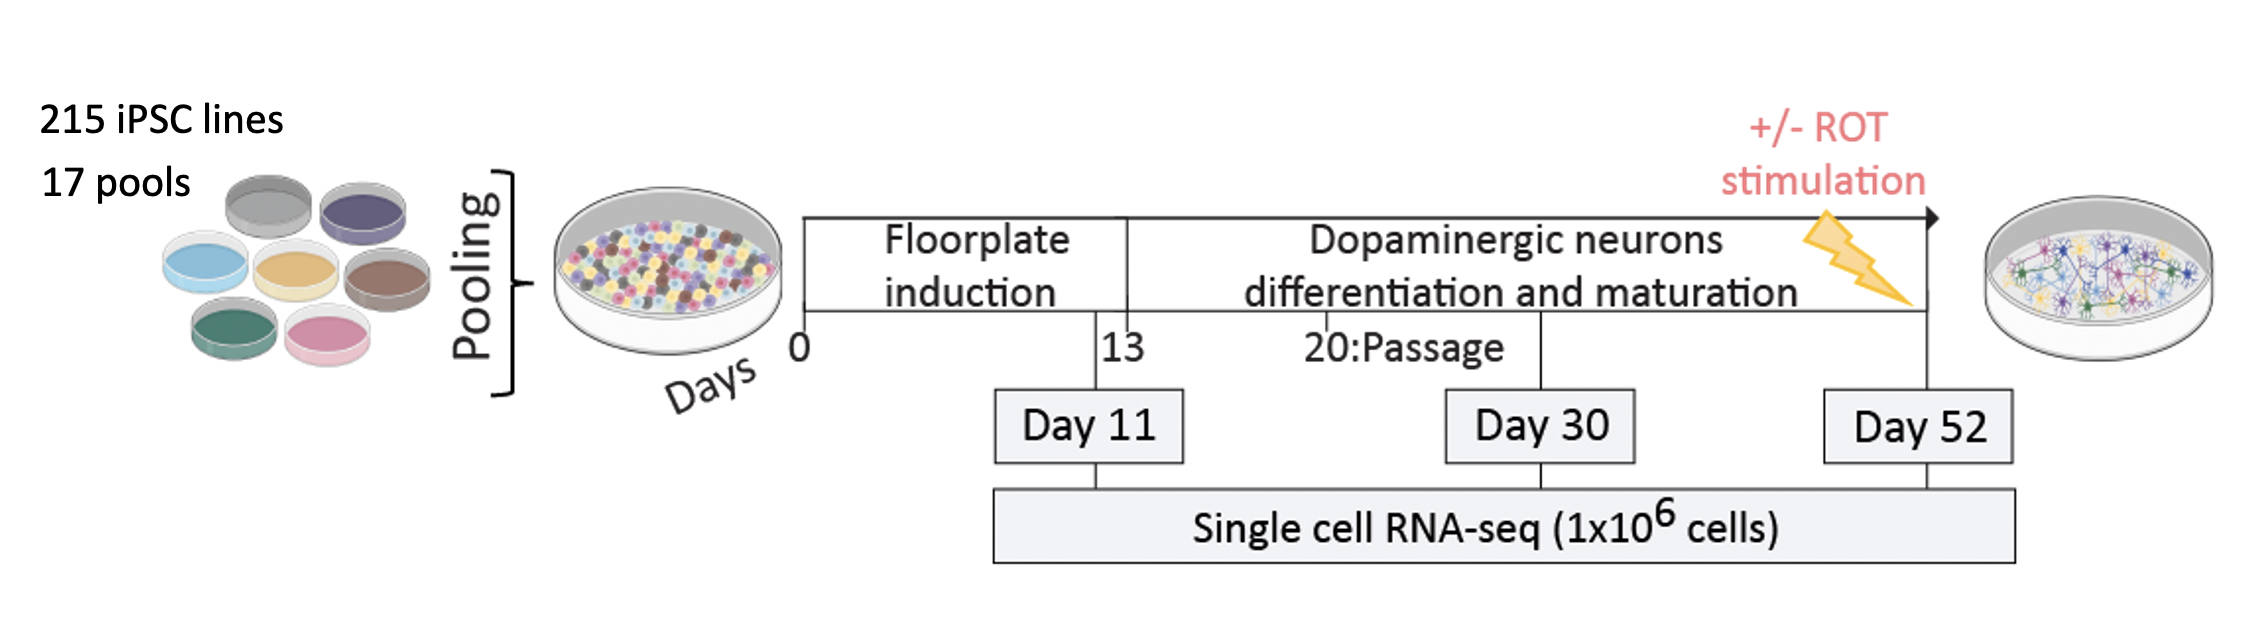
\includegraphics[width=16cm]{Chapter5/Fig/neuroseq_experimental_design.png}
\caption[Experimental Design]{\textbf{Experimental Design}.\\
Figure created by Julie Jerber.
Experimental design for pooled differentiations of iPSC to midbrain dopaminergic neurons. 
The three time points (day 11, day 30, day 52) at which cells were collected for \gls{scrnaseq} profiling are shown. 
On day 51, 50\% of the cells were stimulated with rotenone for 24h, to induce an oxidative stress.
Data from 215 iPSC lines (for 215 donors) across 17 pools were collected for a total of over a million cells.}
\label{fig:neuroseq_experimental_design}
\end{figure}

% \newpage

% \subsection{Neuronal identity}

% % We selected 215 iPSC lines derived from healthy donors by the HipSci project \cite{kilpinen2017common} for differentiation towards a midbrain cell fate, including dopaminergic neurons \cite{kriks2011dopamine}. 
% % Differentiation experiments were multiplexed using pools containing between 7 and 24 cell lines per experiment. 
% Immunochemistry confirmed that cells from both pooled and conventional differentiation of individual lines expressed protein markers associated with patterning of DA (LMX1A, FOXA2 and TH, Fig. \ref{fig:neuroseq_staining}). 
% % To capture transcriptional changes during neurogenesis and neuronal maturation, we performed \gls{scrnaseq} of cells captured at day 11 (day 11, midbrain floorplate progenitors), day 30 (day 30, young post-mitotic midbrain neurons) and day 52 (day 52, more mature midbrain neurons). 
% % To mimic an oxidative stress condition, we also profiled day 52 neurons upon exposure to a sub-lethal dose of rotenone (ROT, 0.1 μM; 24 h) a chemical stressor that preferentially leads to DA death in models of PD \cite{xiong2012mitochondrial}.


% \begin{figure}[h]
% \centering
% 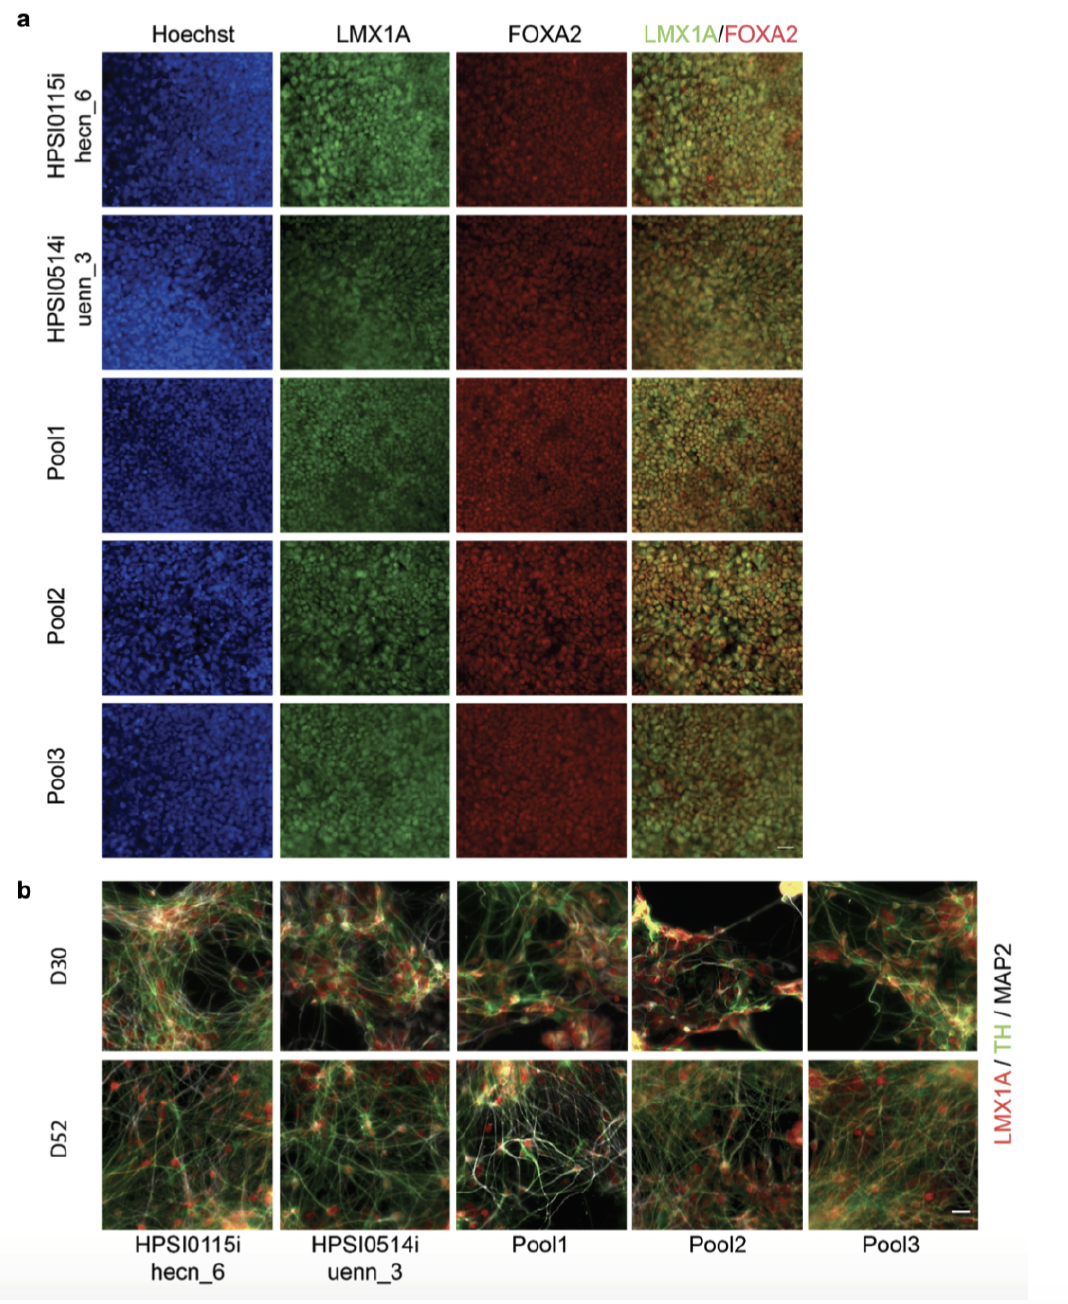
\includegraphics[width=11cm]{Chapter5/Fig/neuroseq_immunostaining.png}
% \caption[Immunostaining of midbrain progenitors and neurons.]{\textbf{Immunostaining of midbrain neural progenitors and dopaminergic neurons}.\\
% Figure created by Julie Jerber.
% (a) Immunostaining for known midbrain progenitor markers LMX1A and FOXA2 at day 11. 
% Nuclei were counter-stained with Hoechst. 
% Scale bar: 25μm. 
% (b) Immunostaining of differentiated dopaminergic neurons for the neuronal marker MAPT2 (white) and the dopaminergic neuronal
% markers TH and LMX1A. 
% Scale bar: 25μm. 
% Data is shown for two example individual cell lines(HPSI0155i-hecn\_6 and HPSI0514i-uenn\_3) as well as three entire differentiation pools (pools 1,2,3).}
% \label{fig:neuroseq_staining}
% \end{figure}

\newpage

% \subsection{Data processing and QC}
\subsection{Demultiplexing donors from pooled experiments}

For each of the 17 pooled experiments, donors (i.e. cell lines) were demultiplexed using demuxlet \cite{kang2018multiplexed}, considering genotypes of common exonic variants (MAF > 1\%) available from the HipSci bank, and a doublet prior of 0.05. 
Only single cells for which donor identification was successful were considered further. 
This QC step filtered out two kinds of droplet: droplets that contained two or more cells from different donors, and droplets containing no cells, but 
% that contained a mixture of 
enough
free-floating RNA 
% and had therefore passed 
to pass
the CellRanger UMI filter.

\subsection{Normalisation, dimensionality reduction, and clustering}

% After QC, we obtained a total of 1,027,401 cells across 19 cell pools and four conditions. 
% The cell line of origin for each cell was inferred from single cell RNA-seq read data using known genotypes made available by the HipSci consortium (using demuxlet, \cite{kang2018multiplexed}). 

Independent analysis of each time point allowed efficient batch effect correction, as all samples were from the same time point, containing similar mixtures of cell types.
Moreover, by reducing the number of cells analysed together, computational tasks were made more tractable.
In particular, the following steps were performed (at each time point): counts were normalised to the total number of counts per cell. 
Next, only genes with non-zero counts in at least 0.5\% of cells were retained and the top 3,000 highly variable genes were selected, after correcting for the mean-variance relationship in expression data. 
The first 50 principal components (PCs) were then calculated, and
batch correction was applied on the level of PCs using Harmony \cite{korsunsky2019fast}, with each 10X sample treated as a distinct batch. 
UMAP and clustering was performed using the resulting transformed PCs. 
In particular, clustering was performed using Louvain clustering \cite{blondel2008fast} with 10 nearest neighbours. 
Data processing steps besides batch correction were performed using the Scanpy package \cite{wolf2018scanpy}. 
This identified a total of 26 clusters (6, 7 and 13 clusters at day 11, day 30, day 52, respectively \textbf{Fig. \ref{fig:neuroseq_clusters}}). \\

% ugly, remake with less space to the left
\begin{figure}[h]
\centering
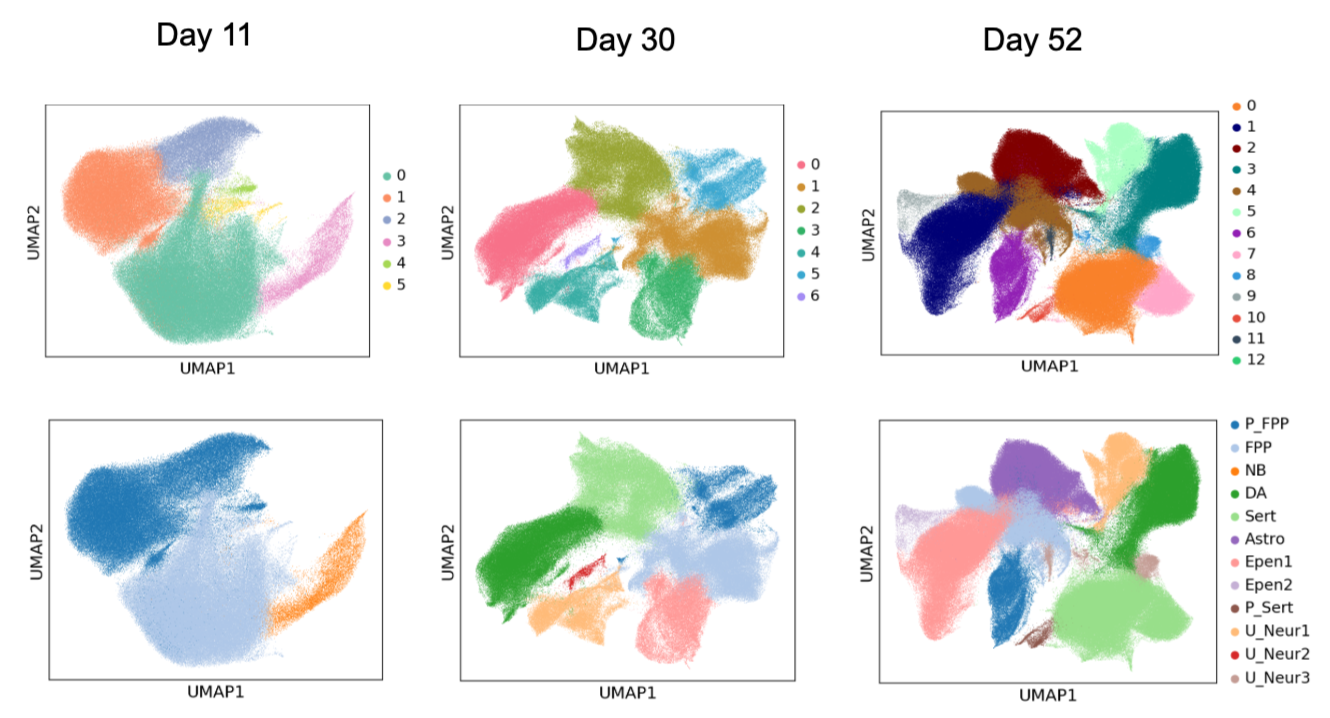
\includegraphics[width=16cm]{Chapter5/Fig/neuroseq_clusters_celltypes.png}
\caption[Clustering and cell type assignment]{\textbf{Clustering and cell type assignment}.\\
At each individual time point (day 11, day 30, day 52), cells were clustered using Louvain clustering \cite{blondel2008fast}, after normalisation and batch correction using Harmony \cite{korsunsky2019fast}.
Subsequently, clusters were annotated as cell types using known marker genes. 
When two clusters showed the same gene set enrichment they were computationally assigned to the same cell type identity. 
(a) UMAPs of cells sampled at each time point and coloured by cell clusters. 
(b) Same UMAPs as in (a), this time coloured by assigned cell types.
Astro: Astrocyte-like, DA: Midbrain dopaminergic neurons, Epen1,Epen2: Ependymal-like, FPP: Floor Plate Progenitors, NB: Neuroblasts, P\_FPP: Proliferating Floor Plate Progenitors, P\_Sert: Proliferating serotonergic-like neurons, Sert: Serotonergic-like neurons, U\_Neur: Unknown Neurons.}
\label{fig:neuroseq_clusters}
\end{figure}

Next, clusters were assigned to cell types using a set of literature-curated marker genes for major brain cell types (n=48 marker genes). 
When two clusters showed the same gene set enrichment, they were assigned the same cell type identity (see next section).

\subsection{Cell type annotation}
% fix this maybe
Cell type annotation was carried out independently at each time point (day 11, day 30, day 52).
For midbrain dopaminergic neurons, which is the target cell type of this protocol, I also performed additional analyses to verify the cell type identity.
In the next section, I describe the mapping from clusters (identified unbiasedly using the entire transcriptome) to cell types (using literature-curated gene markers).
% Among these, we identified six dominant cell types that were making up at least 10\% of the cells at any time point. 

\subsubsection{Day 11}

Three cell type populations were identified at day 11.
The two most prevalent ones, which constituted circa 96\% of all cells at this time point, were classified as proliferating and non-proliferating midbrain floorplate progenitors (both expressing \textit{LMX1A} and \textit{FOXA2} and expressing \textit{MIK67, TOP2A} when proliferating \cite{la2016molecular}).
The third cell population (making up the remaining 4\% of day 11 cells) was labelled a neuroblast (NB) population, based on the expression of pro-neuronal genes \textit{NEUROD1}, \textit{NEUROG2} and \textit{NHLH1} \cite{bertrand2002proneural, lacomme2012neurog2}, \textbf{Fig. \ref{fig:neuroseq_clusters}}).

\subsubsection{Day 30}

At day 30, cells with floorplate progenitor (23\%) and proliferating progenitor (7\%) identity could still be detected, whereas the neuroblast population was not seen any longer.
Additionally, five new cell types were identified.
Four of these additional cell types appeared neuronal and one was non-neuronal, as characterised by the expression (or lack thereof) of the pan-neuronal markers \textit{SNAP25} and \textit{SYT1} \cite{arenas2015make}.
Of the four neuronal populations, two could be assigned to a midbrain neuronal identity.
The first expressed canonical DA markers \textit{NR4A2}, \textit{PBX1}, and \textit{TMCC3} \cite{la2016molecular, park2006acquisition, ramonet2012park9} and was labelled as a population of midbrain dopaminergic neurons (DA, 27\%).
The second cell population expressed some serotonergic neuronal markers (\textit{TPH2, GATA2} \cite{cummings2019serotonergic}) and was categorised as serotonergic-like (Sert, 21\%) neurons. 
One additional large neuronal population (expressing \textit{SNAP25} and \textit{SYT1}), expressed both midbrain DA markers and cortical markers,
% (Fig. ), 
and thus could not be assigned to a specific neuronal identity (Unknown neurons 1, around 8\%).
Finally, one smaller neuronal population (less than 2\%) could also not be assigned to a specific identity (Unknown neurons 2). 
The only non-neuronal cell type identified at day 30 expressed all the classical markers of ependymal cells (Ependymal 1 \cite{campbell2017molecular}, 11\%,\textbf{ Fig. \ref{fig:neuroseq_clusters}}). 

\subsubsection{Day 52}

At day 52, the cell types identified at day 30 were largely recapitulated (\textbf{Fig. \ref{fig:neuroseq_clusters}}).
Floorplate progenitors were present in smaller proportions (13 and 5\%).
In addition to DA, Sert, the mixed neuronal population 1 and the ependymal-like cell population 1, a population of astrocyte-like cells could be identified, which were unique to day 52 (Astrocyte-like \cite{sloan2017human, zhang2016purification}). 
Finally, three additional rare cell types (present in less than 2\% of cells sampled at any time point) were detected, namely a second ependymal-like population (Ependymal 2), a population of proliferating neuronal serotonergic-like cells (Prolif. serotonergic-like neurons), and one additional neuronal population which could not be annotated unambiguously (Unknown neurons 3, \textbf{Fig. \ref{fig:neuroseq_clusters}}). \\

We note that in general, we are careful to clarify that these are \textit{in vitro}-generated cell types, which will not be exactly the same as their \textit{in vivo} counterpart, especially for cell types that were not the target of the protocol used - thus the nomenclature xx-like, e.g. astrocyte-like, and serotonergic-like.
In the next section I discuss this further for the two cell populations which we assigned to a midbrain neuronal identity.

\subsubsection{Serotonergic-like neuronal population}

First, the population we call serotonergic-like was an especially hard one to define.
Serotonergic neurons are located in the same brain region as dopaminergic neurons 
(the midbrain),
% (the substantia nigra), % only DA, Sert are in the raphe nucleus, right below
and share some common functions and gene markers.
However, whilst dopaminergic neurons have been very well characterised, partly because of their involvement in PD, serotonergic neurons have not been studied as much, and there are no well defined markers (at least not in human, whereas there are a few mouse studies \cite{cummings2019serotonergic}).
% TPH1,..
Additionally, there is no \textit{in vivo} single cell reference dataset.
The only study containing a human serotonergic neuron cell population to the best of my knowledge is La Manno \textit{et al}. \cite{la2016molecular}, which contained only 14 cells.
In the same study they also derive midbrain neurons from human iPSCs, but do not obtain any serotonergic neurons.
Since our population expressed some, but not all, canonical serotonergic markers, 
% (figure, maybe supplement?),
we could not unambiguously say that these were serotonergic neurons, hence the name serotonergic-like.

\subsubsection{Dopaminergic neuronal population}

In contrast, human midbrain dopaminergic neurons are much better annotated, and in particular there exist published \textit{in vivo} datasets we can compare to.
% We further confirmed the dopaminergic identity of our DA cells by comparing our data to three  datasets: human iPSC derived dopaminergic neurons and human fetal cells from La Manno et al., 2016 and data from post-mortem donors from Welch et al., 2019. 
Specifically, to confirm the dopaminergic identity of our DA cell population, I compared our cells to three datasets: human iPSC-derived dopaminergic neurons and human fetal cells from La Manno \textit{et al.} \cite{la2016molecular} and substantia nigra samples from post-mortem donors from Welch \textit{et al}. \cite{welch2019single}. \\

To perform the mapping, I performed joint PCA (batchelor::multiBatchPCA) 
% `batch' = query, reference
and batch correction (batchelor::reducedMNN \cite{haghverdi2018batch}) of log-normalised counts (using scater \cite{mccarthy2017scater}) from our data and each of the three reference datasets. 
The set of genes used was the union of 2,000 highly variable genes (HVGs, using the trendVar function from scran) 
% scran's `trendVar' and `decomposeVar' (using pool\_id design matrix)
from our data and 2,000 HVGs from the reference dataset. 
Next, I asked which reference cell each of our cells was most similar to (i.e. ‘mapped to', using BiocNeighbors::queryKNN with k=1 nearest neighbour).\\

I mapped our DA cells to the set of all neurons from each of three datasets.
First, I compared to the La Manno \textit{et al}. iPSC data, and found that
99\% of our DA cells mapped to the `iDAb' population.
Second, to the La Manno \textit{et al}. embryonic data. 
85\% of our DA cells mapped to one of the dopaminergic populations in the reference, i.e. 39\% to `hDA1', 36\% to `hDA2', and 10\% to `hDA0'.
Finally, we mapped our DA cells to the Welch \textit{et al} post-mortem data, and found that for 91\% cells mapped to `NEUROdop', with the remaining 8\% mapping to a population of inhibitory neurons, `NEUROinh1'.
% JCM: Could perhaps interpret the above? SOmething like this provides confidence in the identity of DA neurons from our iPSC differentiation model. Or something like that?
These combined analyses provide confidence in the identity of DA neurons from our iPSC differentiation model.

% When mapped to the set of all neurons from each independent dataset, our DA cells mapped for 99\% (La Manno hiPSC data), 85\% (La Manno embryonic data) and 91\% (Welch post-mortem human SN samples) to dopaminergic neuron populations.\\

% \textbf{Welch et al}

% comparison 1: all vs all

% 3,419 common genes
% 79\% of our DA cells mapped to the 'NEUROdop' population from \cite{welch2019single} 
% 13\% to NEUROinh1, 4\% to ENDOmural

% 75\% for DA D30 (14\% to NEUROinh1), 92\% for DA D52 untreated, 60\% for DA D52 ROT treated (30\% to NEUROinh1).\\

% comparison 2: neurons (DA, Sert, CHem) vs neurons (grep("NEURO"))

% 3,309 common genes.
% 91\% of our DA cells mapped to the 'NEUROdop' population from \cite{welch2019single}, 8\% to NEUROinh1. 

% 82\% for DA D30 (16\% to NEUROinh1), 99\% for DA D52 untreated, 96\% for DA D52 ROT treated.\\

% \textbf{La Manno et al (human embryo)}

% \cite{la2016molecular}

% comparison 3: all vs all

% 3,023 common genes.

% DA map to hOMTN (33\%), Unknown (26\%), before DA (7\%) or Sert (10\%). \\

% comparison 4: neurons (DA, Sert, CHem) vs midbrain neurons (hDA, hSert)

% 3,260 common genes.

% 11,698/29,801 (39\%) and 10,623/29,801 (36\%) all DA cells map to hDA1 and hDA2, respectively; 15\% hSert, 10\% hDA0.

% 7,913/13,799 (57\%) DA D30 cells map to hDA2, 21\% hDA1, 9\% hSert, 12\% hDA0.

% 6,517/10,947 (60\%) DA D52 NONE cells map to hDA1, 17\% hDA2, 17\% hSert, 6\% hDA0.
% 2,221/5,055 (44\%) DA D52 ROT cells map to hDA1, 18\% hDA2, 28\% hSert, 10\% hDA0.
% \\


% \textbf{La Manno et al (human iPSCs)}

% comparison 5: all vs all

% 3,087 common genes.

% 43\% all DA cells map to iDAb, 19\% iMN1, 12\% iMN2, 10\% iProg2,
% and 87\% day 42, 13\% day 63.

% 39\% DA D30 map to iDAb, 24\% to iMN1, 11\% to iProg2, and 97\% cells map to day 42 cells

% 46\% DA D52 NONE to iDAb, 18\% to iMN1, 9\% to iProg2, and 20\% to iMN2
% and 81\% cells map to day 42 cells, 19\% to day 63 cells

% 46\% DA D52 ROT to iDAb, 11\% to iMN1, 11\% to iProg2, and 26\% to iMN2
% and 73\% cells map to day 42 cells, 27\% to day 63 cells
% \\

% comparison 6: neurons (DA, Sert, CHem) vs iPS neurons (iDA)

% 3,113 common genes.

% 99\% all DA cells mapped to iDAb (over iDAa, iDAc) and 99\% to day 42 (vs day 63).

% 99\% DA D30 cells mapped to iDAb (over iDAa, iDAc) and 99\% to day 42 (vs day 63).

% 99\% DA D52 NONE cells mapped to iDAb (over iDAa, iDAc) and 99\% to day 42 (vs day 63).
% 97\% DA D52 ROT map to iDAb (3\% to iDAc), and 97\% to day 42 (3\% to day 63).

% \begin{Abstract}
% \textbf{Cell type notation}

% DA: dopaminergic neurons;
% Sert: serotonergic neurons;
% FPP: floor plate progenitors;
% P\_FPP: proliferating floor plate progenitors;
% NB: neuroblasts;
% Epen1: ependymal-like cells;
% Astro: astrocyte-like cells
% \end{Abstract}

\newpage

\subsection{Data overview}

For visualisation purposes, we also performed a combined analysis of a random subsample of 20\% of all cells (after QC) from the three time points.
In this case, the Harmony batch correction was performed across pools (rather than across individual 10X samples, as before).
A joint UMAP projection of cells collected across all time points, stimuli and lines revealed broad co-clustering of cell types (using the labels described previously, see \textbf{Fig \ref{fig:neuroseq_clusters}}), but with noticeable differences between time points and stimuli (\textbf{Fig. \ref{fig:neuroseq_overview}}). \\

Substantial variation in the cell type proportions could be observed, across time points and stimuli (\textbf{Fig. \ref{fig:neuroseq_overview}}). 
For example, the proportion of DA cells was significantly reduced upon rotenone stimulation (30\% reduction, Fisher’s exact test, p value = $2.2 \times 10^{-16}$), which was consistent with previous observations that dopaminergic neurons are most affected by apoptosis due to oxidative stress \cite{sherer2003mechanism, knonagel1992autologous, cannon2009highly}.
Collectively, our population-scale \gls{scrnaseq} analysis revealed a diverse repertoire of cell types, enabling both the study of cell line differentiation propensity (\textbf{sections \ref{sec:neuroseq_diff_eff}, \ref{sec:neuroseq_ips}}) and the identification of genetic variants that affect expression in a cell type-specific manner (\textbf{sections \ref{sec:neuroseq_eqt}, \ref{sec:neuroseq_coloc}}). 
\\ 

\begin{figure}[h]
\centering
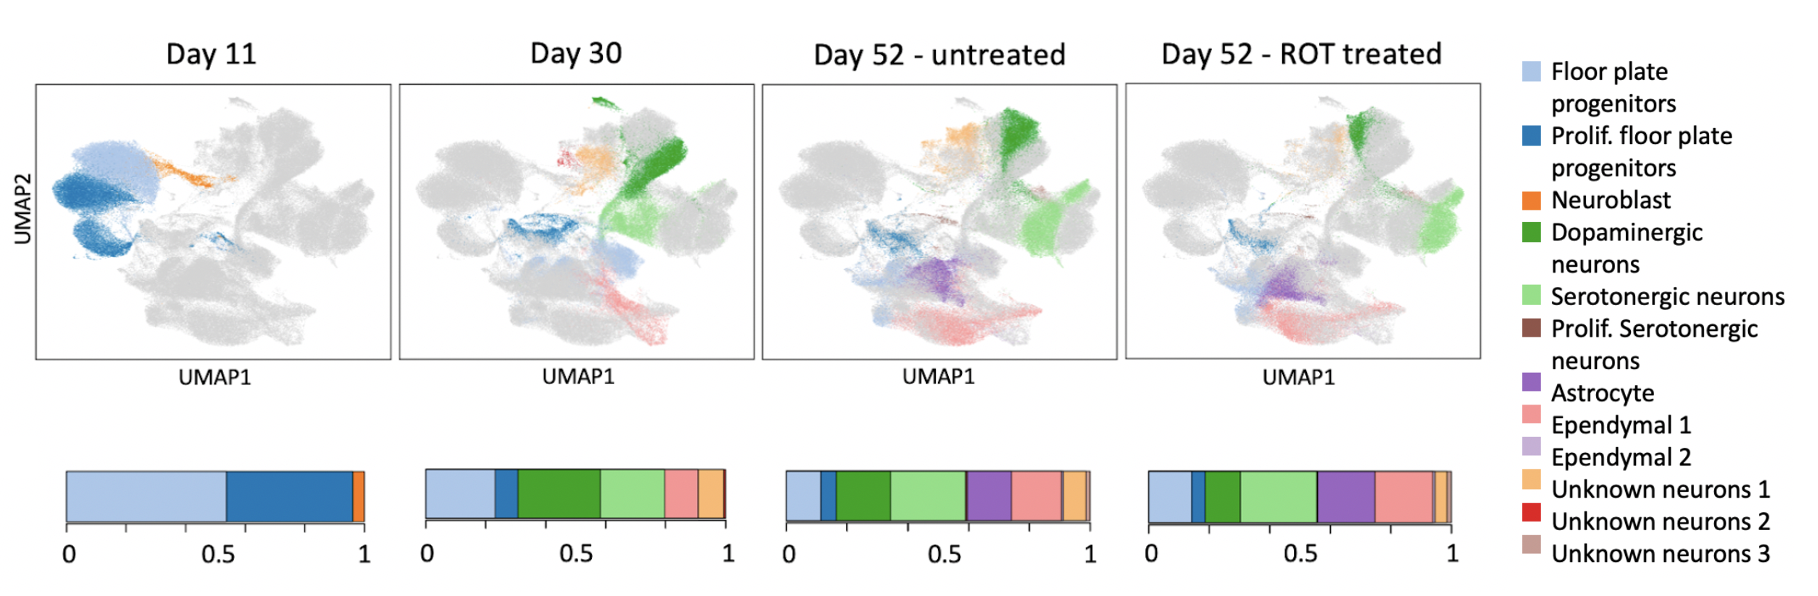
\includegraphics[width=17cm]{Chapter5/Fig/neuroseq_overview.png}
\caption[Overview of study]{\textbf{Overview of study}.\\
Top: UMAP plots of all 1,027,401 cells assayed, coloured by 
% annotated 
cell type identity. 
Cells that were not collected at a given (time point, stimulus) condition are shown in light grey. 
Prolif: Proliferating. 
Bottom: Bar plots showing, for each condition, the fraction of cells assigned to each cell type.}
\label{fig:neuroseq_overview}
\end{figure}

% Add here neuronal maturation index?

\newpage

\section{Line-to-line variation in neural differentiation efficiency}
\label{sec:neuroseq_diff_eff}

% OS: Feels a bit disconnectd to CH4 where you have the same refs / point. connect.
The great diversity of cell types generated by this protocol raised the question of whether it may be driven by variation in differentiation outcome between different iPSC lines, which, as we have seen, is prevalent in iPSC differentiation studies (see \textbf{section \ref{sec:endodiff_differentiation_efficiency}} as well as other studies e.g. \cite{d2019association, volpato2018reproducibility}). 
Yet, as we discussed, the biological basis for this high variability in differentiation outcomes between lines remains largely obscure, which complicates efforts to rationally select cell lines for different applications. 
Here, we found substantial variation in the proportions of different cell types produced by different iPSC cell lines at each time point. 
For example, the proportion of day 52 untreated cells assigned to DA neurons ranged from 1\% to 100\% from line to line.
(\textbf{Fig. \ref{fig:neuroseq_line_variation}}).
% \\

\begin{figure}[h]
% \centering
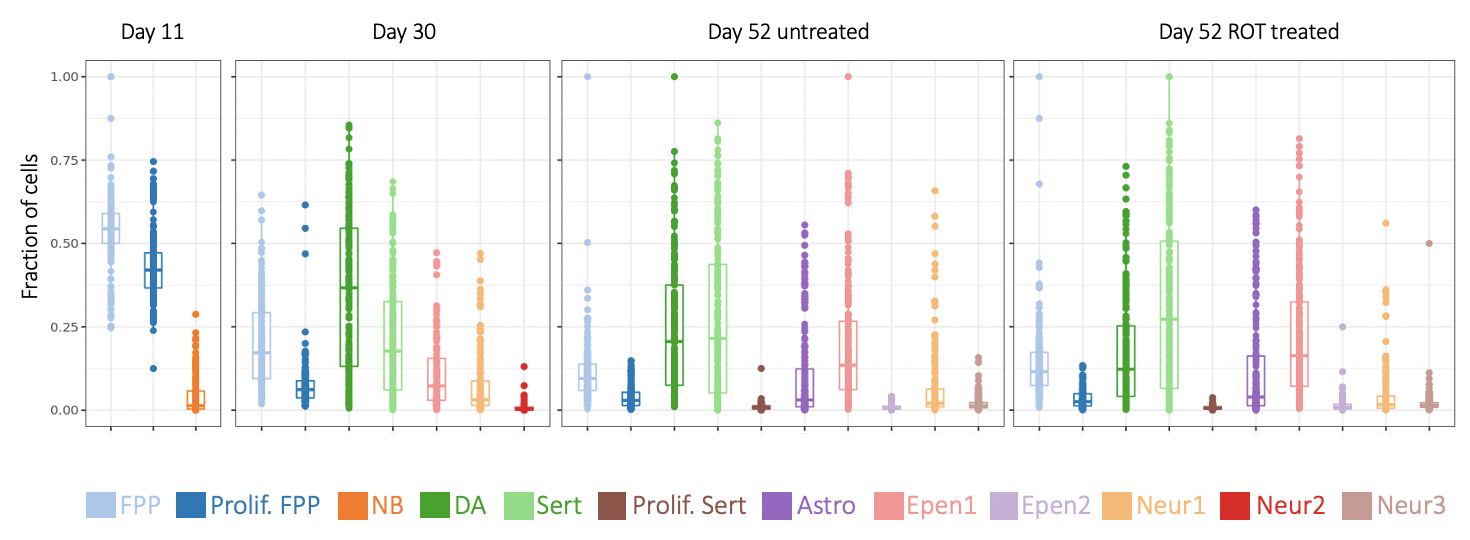
\includegraphics[width=15.5cm]{Chapter5/Fig/neuroseq_line_celltype.png}
\caption[Cell type fractions across lines]{\textbf{Cell type fractions across lines}.\\
Box plots showing, for each cell type, the proportions of that cell type across cell lines at day 11, day 30, untreated day 52, rotenone-treated day 52. 
Each point indicates a different cell line.}
\label{fig:neuroseq_line_variation}
\end{figure}

% \clearpage

Looking at the cell type fractions per cell line and pool across time points, we observed a bimodality in the data, with roughly 2/3 of the iPSC lines mostly making DA and Sert at day 30 and day 52, and the other 1/3 making very few midbrain neurons but many glial cells (Ependymal-like and Astrocyte-like) instead (\textbf{Fig. \ref{fig:neuroseq_diff_efficiency}}).
When we performed \gls{pca} of such cell type fractions matrix, we identified the proportion of midbrain neurons (DA and Sert) on day 52 as the largest axis of variation (PC1, 47\% variance, \textbf{Fig. \ref{fig:neuroseq_diff_efficiency}}). 
Since DA and Sert cells are derived from similar progenitor populations \textit{in vivo}, it is not surprising that both populations are observed in our differentiation experiment \cite{ye1998fgf, cao2017characterization}. 
This motivated us to estimate a `neuronal differentiation efficiency' for each iPSC line, defined as the sum of the fractions of DA and Sert cells produced on day 52 (\textbf{Fig. \ref{fig:neuroseq_diff_efficiency}}). 
\\

\begin{figure}[htbp]
\centering
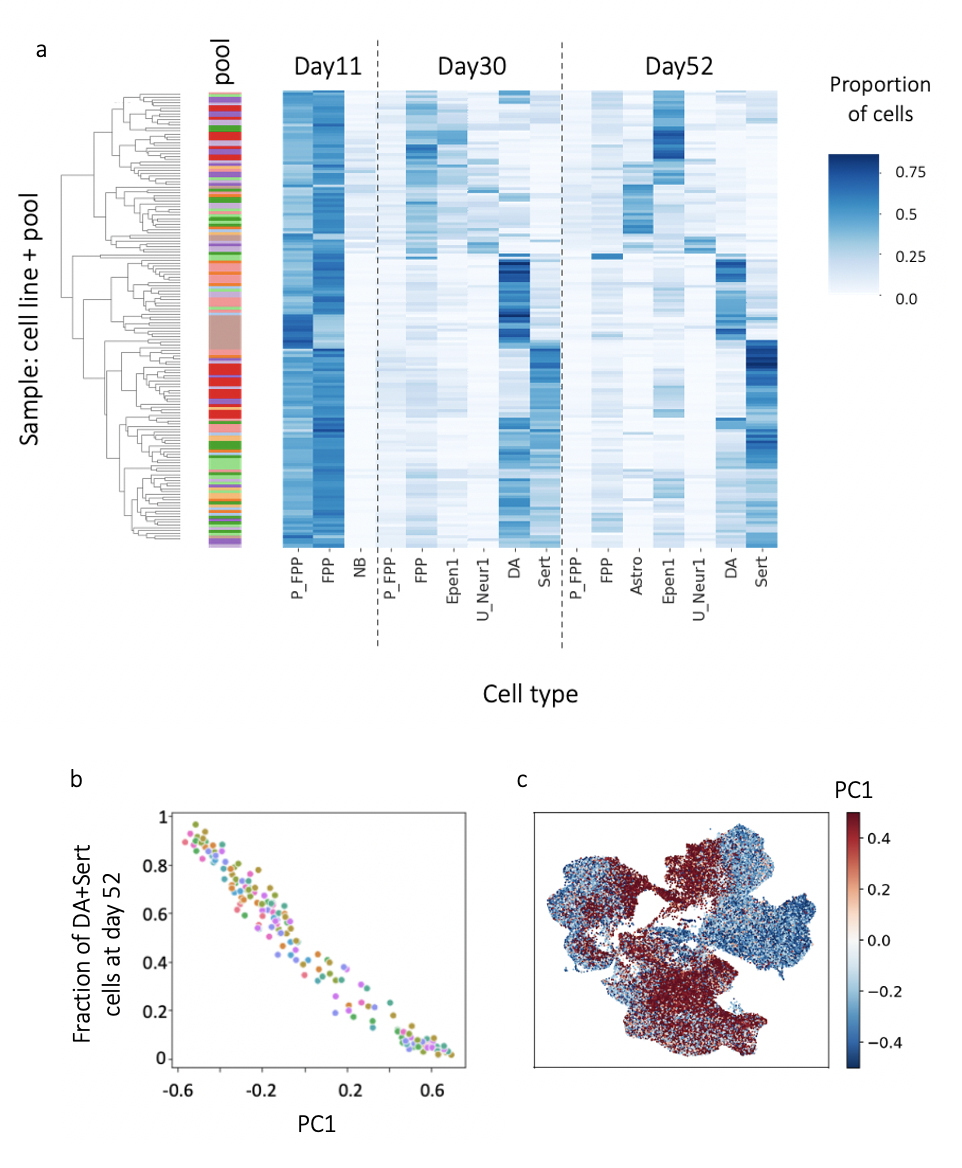
\includegraphics[width=14cm]{Chapter5/Fig/neuroseq_define_diff_efficiency.png}
\caption[Definition of neuronal differentiation efficiency]{\textbf{Distribution of cell proportions at day 52 and definition of neuronal differentiation efficiency}.\\
Cell proportions were generated for each cell type and time point for all combinations of cell lines and pools with at least 10 cells at all time points (10 pools). 
(a) Heatmap of the resulting cell proportion matrix. 
Pools are shown in the first bar and the colours indicate in which of the 10 pools each line was differentiated. 
Rows (i.e. cell line, pool combinations) were hierarchically clustered according to Euclidean distance. 
(b) Comparison of the first principal component (PC1) to the sum of fractions of dopaminergic and serotonergic-like neurons present on day 52.
(c) UMAP of cells included in (a), coloured by PC1.}
\label{fig:neuroseq_diff_efficiency}
\end{figure}

\clearpage

We assessed the reproducibility of this measure of neuronal differentiation efficiency using data from 32 lines that were differentiated twice, in two different pools. 
Importantly, we found that iPSC line neuronal differentiation efficiency defined in this way was highly reproducible between different pools (Pearson's R = 0.75; p value = $2 \times 10^{-6}$, \textbf{Fig. \ref{fig:neuroseq_diff_eff_replication}}).

\begin{figure}[h]
\centering
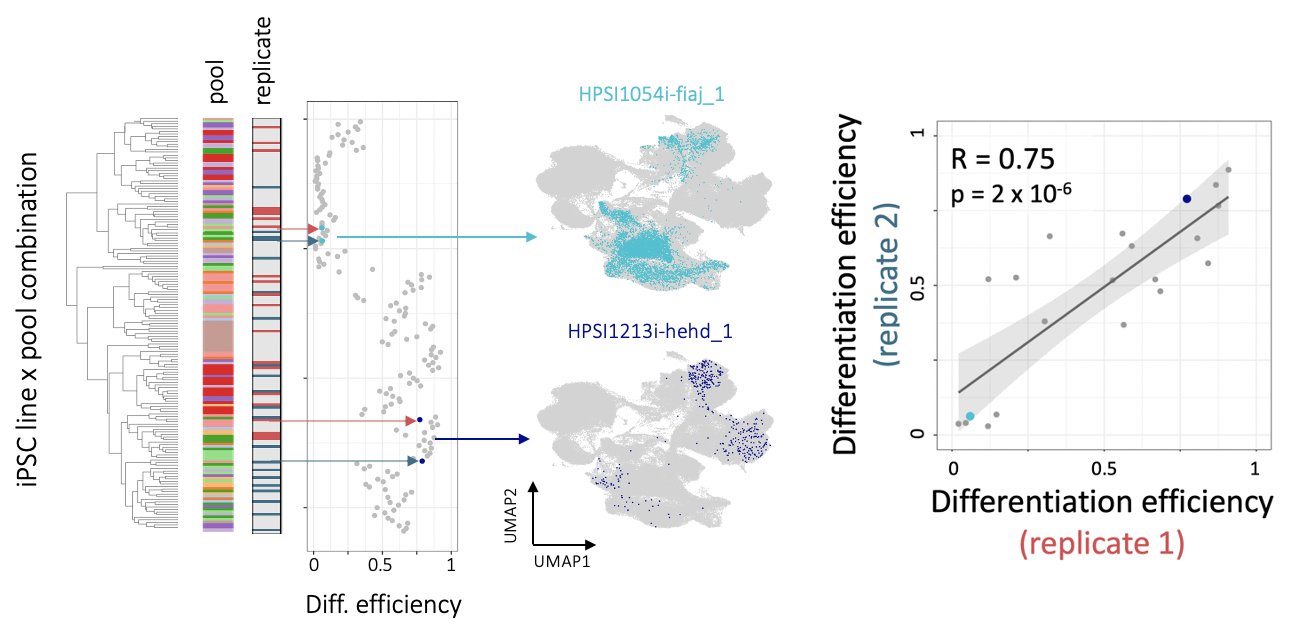
\includegraphics[width=15.5cm]{Chapter5/Fig/neuroseq_diff_eff_replication.png}
\caption[Reproducible neural differentiation efficiency]{\textbf{Reproducible variation in differentiation trajectories}.\\
(left) Hierarchical clustering of (cell line, pool) combinations (same as \textbf{Fig. \ref{fig:neuroseq_diff_efficiency}}) by neural differentiation efficiency. 
Colours in the first bar indicate in which of 10 pools (for which we had data at all time points, used to define neuronal differentiation efficiency) each line was differentiated. 
Differentiation replicates for lines present in two pools, are indicated in the second bar (red for replicate 1 blue for replicate 2).
(middle) UMAPs, highlighting the distributions of cells on day 52 for two selected cell lines with low and high differentiation efficiencies respectively (HPSI0514i-fiaj\_1, in seagreen and HPSI1213i-hehd\_1, in dark blue).
(right) Scatter plot showing estimated neuronal differentiation efficiency between differentiation replicates (i.e. cell lines differentiated in two different pools, out of the 10 pools considered here, n=21). 
Highlighted are the same two cell lines.}
\label{fig:neuroseq_diff_eff_replication}
\end{figure}

% \clearpage

\subsection{Organoids}
Given the robustness of our measure of neuronal differentiation efficiency, we next wondered if it was generalisable to other differentiation approaches. 
We therefore differentiated a pool of 18 lines (pool 4) into cerebral organoids for 113 days (as previously described in Lancaster \textit{et al}. \cite{lancaster2017guided}) and profiled the resulting cell populations using \gls{scrnaseq} (11,445 cells). 
The same steps of dimensionality reduction, batch correction and clustering applied to the midbrain dataset were applied to the cerebral organoid data. 
These steps identified eight clusters that were labelled as different cell types (i.e. neuronal cells, intermediate progenitor cells, radial glial progenitor cells, satellite cells, mesenchymal cells, myotube and Wnt and PAX7 positive cells) using 24 marker genes (\textbf{Fig. \ref{fig:neuroseq_organoids}}).
We found that the proportion of brain cell types (all neuronal, glial, and neural progenitor cells) produced by each line in the cerebral organoids was strongly correlated with neuronal differentiation efficiency as estimated from the dopaminergic differentiation (R = 0.94; p value = $2 \times 10^{-5}$; n=12). 
Taken together, these results strongly suggest that variation in iPSC neuronal differentiation efficiencies arise primarily due to cell-intrinsic factors. 
Furthermore, the consistency of neuronal differentiation efficiency suggests that these properties extend to neuronal differentiation more generally.
% \\

\begin{figure}[htbp]
\centering
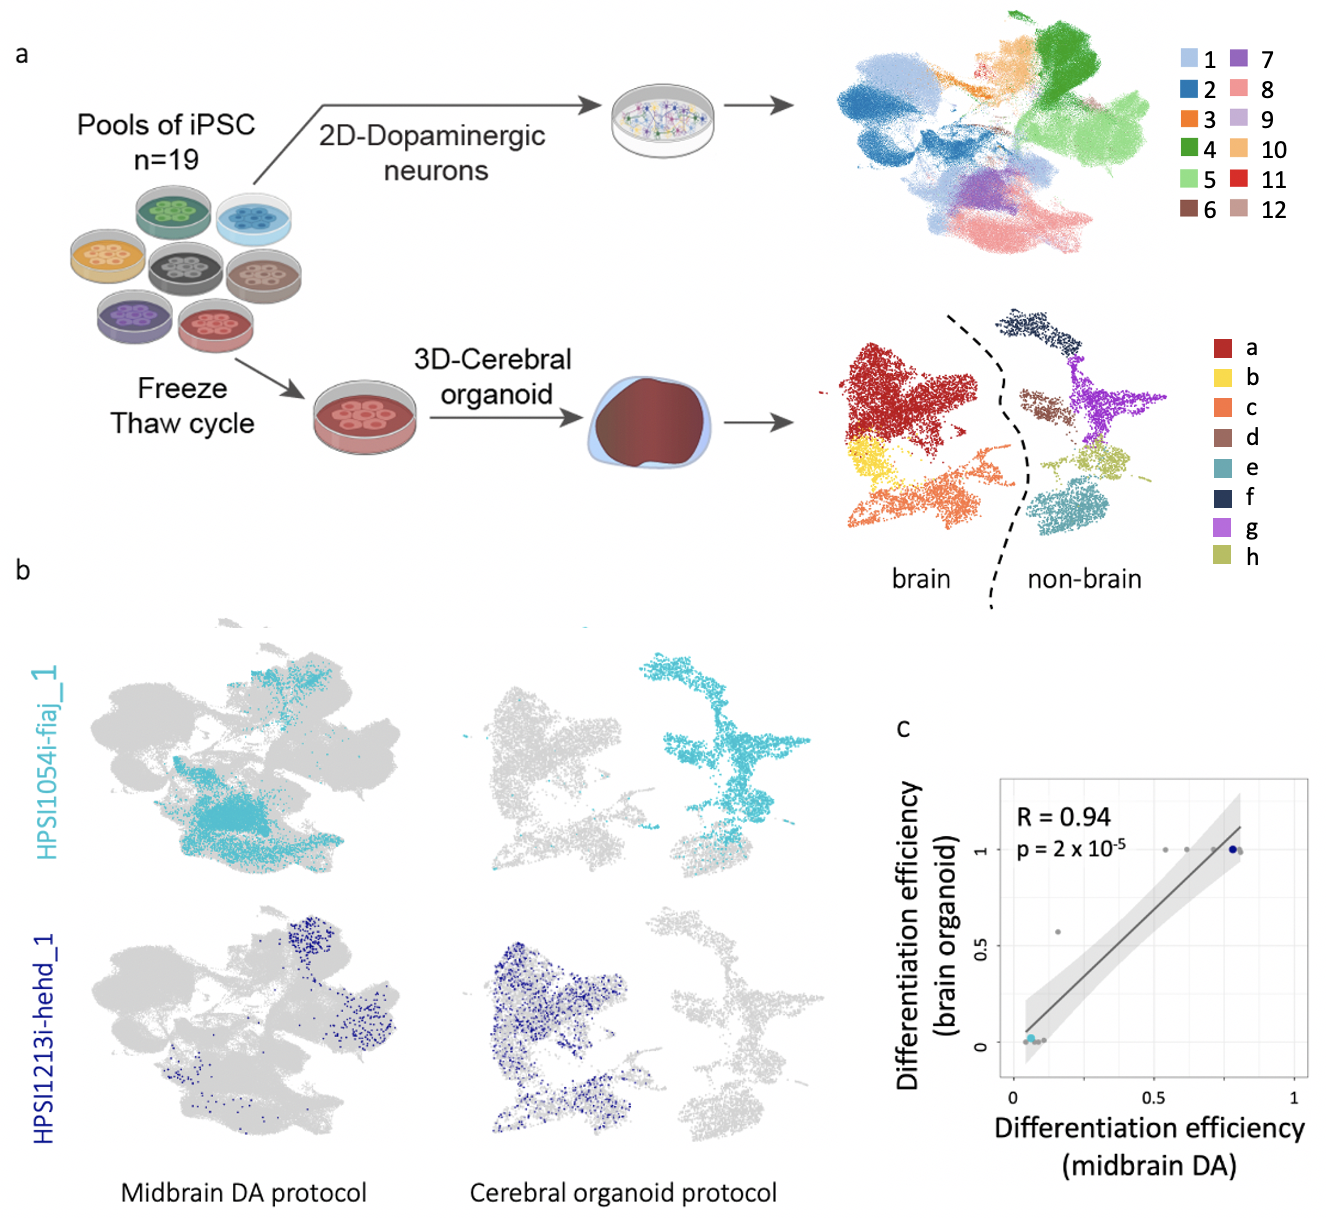
\includegraphics[width=14cm]{Chapter5/Fig/neuroseq_organoids.png}
\caption[Neuronal differentiation efficiency in cerebral organoids]{\textbf{Neuronal differentiation efficiency in cerebral organoids}.\\
(a) Experimental workflow for single cell profiling of iPSC-derived cerebral organoids using one pool containing 18 cell lines, profiled using scRNA-seq after 113 days of differentiation.
% Add cell type legend. 
(b) UMAPs of two representative cell lines making non-brain and brain cell types in the organoid study. 
(c) Scatter plot of neuronal differentiation efficiency as measured using midbrain dopaminergic neuronal differentiation (x-axis) versus neural differentiation efficiency as measured in organoid differentiation (y-axis) for a subset of 12 iPS cell lines in common. 
Highlighted are the same two cell lines as in (b).}
\label{fig:neuroseq_organoids}
\end{figure}

% In contrast, when compared to the endoderm differentiation efficiency defined in the previous chapter (for the lines shared between the two studies, n = 45), we found no correlation, suggesting that different germ layers..

\clearpage

\section{iPSC expression can predict neuronal differentiation efficiency}
\label{sec:neuroseq_ips}

Motivated by the reproducibility of differentiation outcomes across multiple independent pools, we set out to explore possible predictors (similar to the analysis described in \textbf{section \ref{sec:endodiff_differentiation_efficiency}}).
The idea was that, if we could find characteristics that could be measured in iPSCs and that would predict 
% in particular 
a bad differentiation outcome, they could become a 
% very 
useful tool to select the most suitable lines prior to differentiation. \\

We began by testing for associations between neuronal differentiation efficiency and other experimental and biological factors.
Those included cell line passage number (p value = 0.77), donor sex (p value = 0.008), chromosome X activation status (p value = 0.01), and PluriTest scores \cite{muller2011bioinformatic} (p value = 0.01).
Although some of these were nominally significant, they explained little variation as compared to line-specific effects, when we performed variance component analysis, by modelling:

\begin{equation}\label{eq:neuroseq_vca}
    \mathrm{neuronal \ differentiation \ efficiency = Donor/Line + Pool + Sex + Age + \boldsymbol{\psi}},
\end{equation}

where Line (which cannot be distinguished from Donor), Pool, Sex and Age are all modeled as random effects (n=230 line-pool combinations).
To assess specifically the effect of X chromosome inactivation status, we fitted an alternative model which was limited to the female donors (n=115 line-pool combinations):

\begin{equation}\label{eq:neuroseq_vca_xci}
    \mathrm{neuronal \ differentiation \ efficiency = Donor/Line + Pool + XCI + Age + \boldsymbol{\psi}}. 
\end{equation}

\begin{figure}[htbp]
\centering
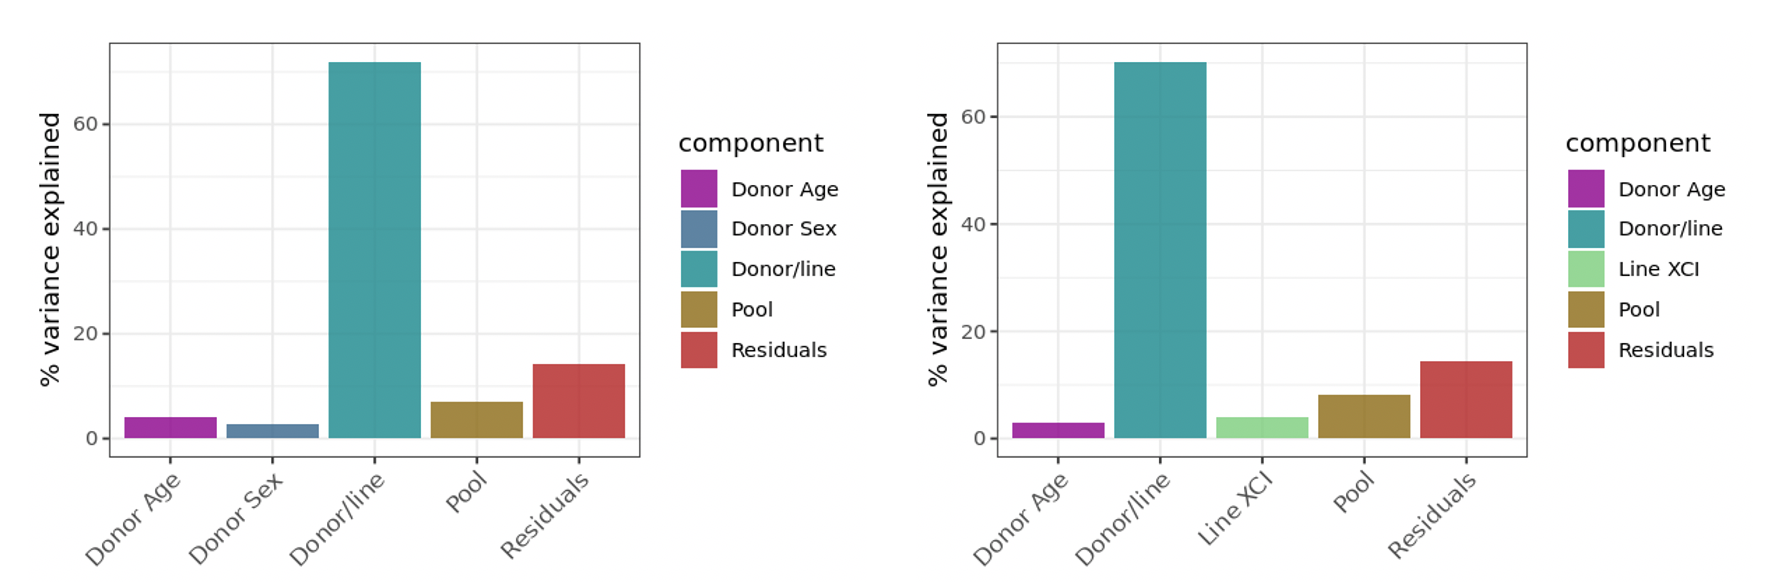
\includegraphics[width=16cm]{Chapter5/Fig/neuroseq_diff_eff_vca.png}
\caption[Variance component analysis of neuronal differentiation efficiency]{\textbf{Variance component analysis of neuronal differentiation efficiency}.\\
Results from variance component models in eq. \eqref{eq:neuroseq_vca} and \eqref{eq:neuroseq_vca_xci}, respectively.
The variance explained by each component was re-scaled to sum up to 100.
% describe how it's measured? XCI
XCI is categorised into 0.1-wide bins: [0-0.1]..[0.4-0.5].}
\label{fig:neuroseq_diff_eff_vca}
\end{figure}

\newpage

% OS: again more context to ch ch4
We note that there is some effect of the technical batch iPSC lines were differentiated in, as it has been observed before \cite{kilpinen2017common, schwartzentruber2018molecular}, yet line-specific effects are prevalent (\textbf{Fig. \ref{fig:neuroseq_diff_eff_vca}}).
This is confirmed when we consider data from 6 lines (from pools 1, 2 and 3) that were differentiated individually, as well as in pools.
When we compared our measure of neuronal differentiation efficiency for each of the lines when differentiated alone or in a pool, we found strongly concordant results (R = 0.83, p value = 0.034).\\ 

Next, we assessed whether neuronal differentiation efficiency was associated with particular patterns of gene expression in undifferentiated iPSCs. 
Using data from independent bulk RNA-seq data available for a subset of 184 iPSC lines included in this study \cite{kilpinen2017common, bonder2019systematic} we identified significant associations with neuronal differentiation efficiency for 2,045 genes (983 positive and 1,062 negative associations; F-test, FDR < 5\%, \textbf{Fig. \ref{fig:neuroseq_ips_expression_signature}}). 

\begin{figure}[h]
\centering
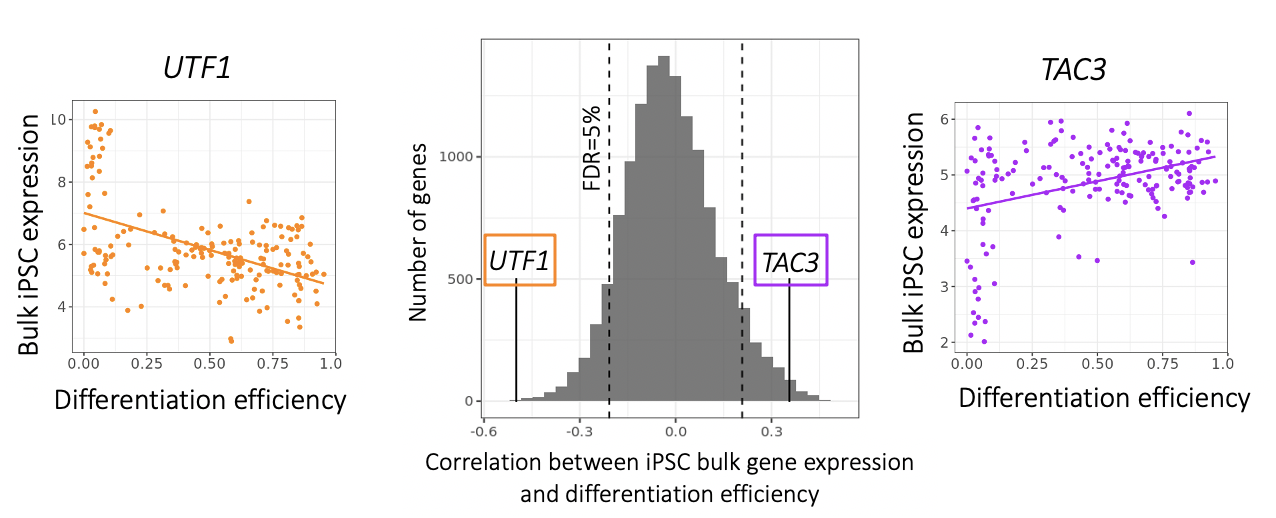
\includegraphics[width=16cm]{Chapter5/Fig/neuroseq_ips_bulk_expr_correlations.png}
\caption[iPS expression signature of neuronal differentiation efficiency]{\textbf{An iPSC expression signature is associated with neuronal differentiation efficiency}.\\
Histogram of Pearson correlation coefficients between iPSC gene expression of individual genes (measured using bulk RNA-seq \cite{bonder2019systematic}) and neuronal differentiation efficiency. 
Two exemplar genes (\textit{UTF1, TAC3}) are highlighted. 
\textit{UTF1} is an example of a gene whose expression level in iPSC (based on bulk RNA-seq) is negatively correlated with neuronal differentiation efficiency (R = -0.5, p value = 3.5$ \times 10^{-13}$ ), whereas \textit{TAC3} is positively correlated (R = 0.38, p value = 9.8$ \times 10^{-8}$).}
\label{fig:neuroseq_ips_expression_signature}
\end{figure}

\newpage

\subsection{A predictor of (poor) differentiation using iPSC gene expression}

The examples shown in \textbf{Fig. \ref{fig:neuroseq_ips_expression_signature}} suggest that differentiation potential and especially poor differentiation (< 0.2) may be associated with clear expression signatures.
Motivated by this observation, we used the genome-wide gene expression signature in undifferentiated iPSCs to build a model to predict poor differentiation outcomes, where we defined poor differentiation as a binary outcome (neuronal differentiation efficiency < 0.2).
We used a logistic regression and obtained 100\% precision at 35\% recall as assessed by cross-validation. 
This result was robust to alternative thresholds for defining poor differentiation outcomes (\textbf{Fig. \ref{fig:neuroseq_diff_eff_predictor}}). 

\begin{figure}[h]
\centering
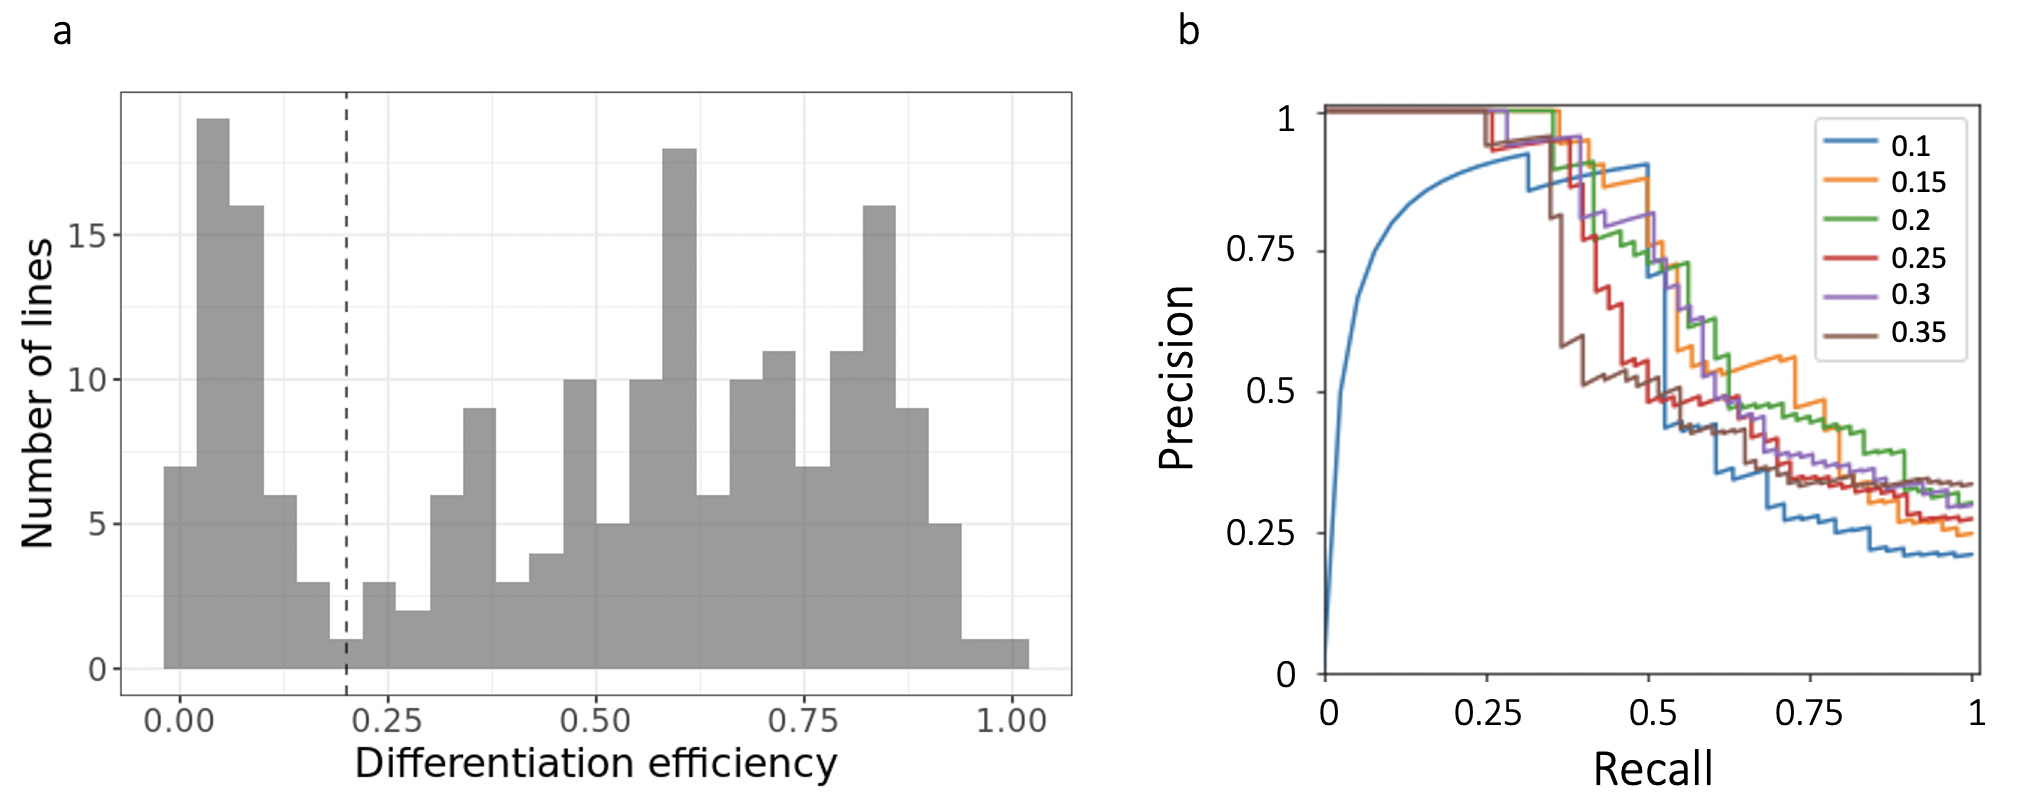
\includegraphics[width=15.5cm]{Chapter5/Fig/neuroseq_diff_eff_predict.png}
\caption[Predicting differentiation failure from iPSC gene expression]{\textbf{Predicting differentiation failure from iPSC gene expression}.\\
(a) Histogram of neuronal differentiation efficiencies across cell lines. 
The threshold chosen to define differentiation success or failure (i.e. neuronal differentiation efficiency = 0.2) is shown by the dashed line, separating the two modes of the distribution. 
(b) Precision-recall curves for a logistic regression model predicting differentiation failure from iPSC gene expression data \cite{bonder2019systematic} using a range of thresholds between 0.1 and 0.35 to define differentiation failure. 
Results are presented from leave-one-out cross validation.}
\label{fig:neuroseq_diff_eff_predictor}
\end{figure}

We then used this model to generate predicted scores for all 812 HipSci lines for which bulk RNA-seq data was available.
This analysis indicated that a substantial fraction of lines in the HipSci resource (26\%) were predicted to produce < 20\% neuronal cells under the differentiation conditions we tested.
Furthermore, we tested whether the same experimental and biological factors previously associated with neuronal differentiation efficiency replicated in this larger sample and found consistent results.
Finally, we did not observe strong concordance between the predicted differentiation outcomes of different cell lines from the same donor, suggesting that donor genetic background is unlikely to play an important role in driving differentiation biases (\textbf{Fig. \ref{suppl_fig:predicted_scores_donors}}).

% chi square test compared to proportions of concordant/discordant expected by change, p=0.1991
% (neither of these two last points are shown, and neither is the validation performed upon revision. Add?)
% figure?

\newpage

\subsection{A subpopulation of iPSCs is associated with poor differentiation}

Next, 
% since iPSC cultures are heterogeneous, 
we hypothesised that the predictive gene expression signature identified in bulk RNA-seq at iPSC state may reflect variation in the proportion of subpopulations in iPSCs. 
To test this hypothesis, we re-analysed scRNA-seq data from 112 iPSC lines that were assayed previously under iPSC culture conditions similar to those used here \cite{cuomo2020single}, 45 of which were also included in this study)\footnote{This is the day 0 population from the data presented in \textbf{Chapter \ref{chapter4}}, and the same iPSC single cell population used in \textbf{Chapter \ref{chapter3}}.}. 
After processing the data using the same pipeline as used above (i.e. Harmony batch correction, Louvain clustering),
we identified 5 clusters, 
% all but one of 
which expressed similarly high levels of core pluripotency markers (\textit{NANOG, SOX2, POU5F1}, \textbf{Fig. \ref{fig:neuroseq_ips_sc_genes}}). \\

We found that genes whose expression predicted poor differentiation (e.g. \textit{UTF1}) were highly enriched in one of those clusters (cluster 2), while genes whose expression were predictive of successful differentiation (e.g. \textit{TAC3}), were down-regulated in cluster 2 relative to the remaining iPSC clusters (\textbf{Fig. \ref{fig:neuroseq_ips_sc_genes}}). 
% In comparison, other cell clusters did not show such equivalent enrichment in differentiation marker genes.
% \\
As a validation of this hypothesis, we also tested for and confirmed a significant association between the fraction of cells in cluster 2 and neuronal differentiation efficiency for each cell line (Pearson R = -0.76, p value = $2.05 \times 10^{-9}$, \textbf{Fig. \ref{fig:neuroseq_ips_sc_genes}}). 
We used additional data from \cite{cuomo2020single} to assess the consistency of the portion of cluster 2 cells across replication experiments, finding good concordance (Pearson R = 0.9; n=23, \textbf{Fig. \ref{fig:neuroseq_ips_sc_genes}}).
Using the known relationship between iPSC bulk RNA-seq and the proportion of cluster 2 cells, we predicted this proportion for 182 cell lines included in our differentiation experiments, and confirmed the negative correlation with neuronal differentiation efficiency (Pearson R = -0.49; p value = $3 \times 10^{-12}$, \textbf{Fig. \ref{suppl_fig:ipsc_cluster2}}). 
\\

\begin{figure}[htbp]
\centering
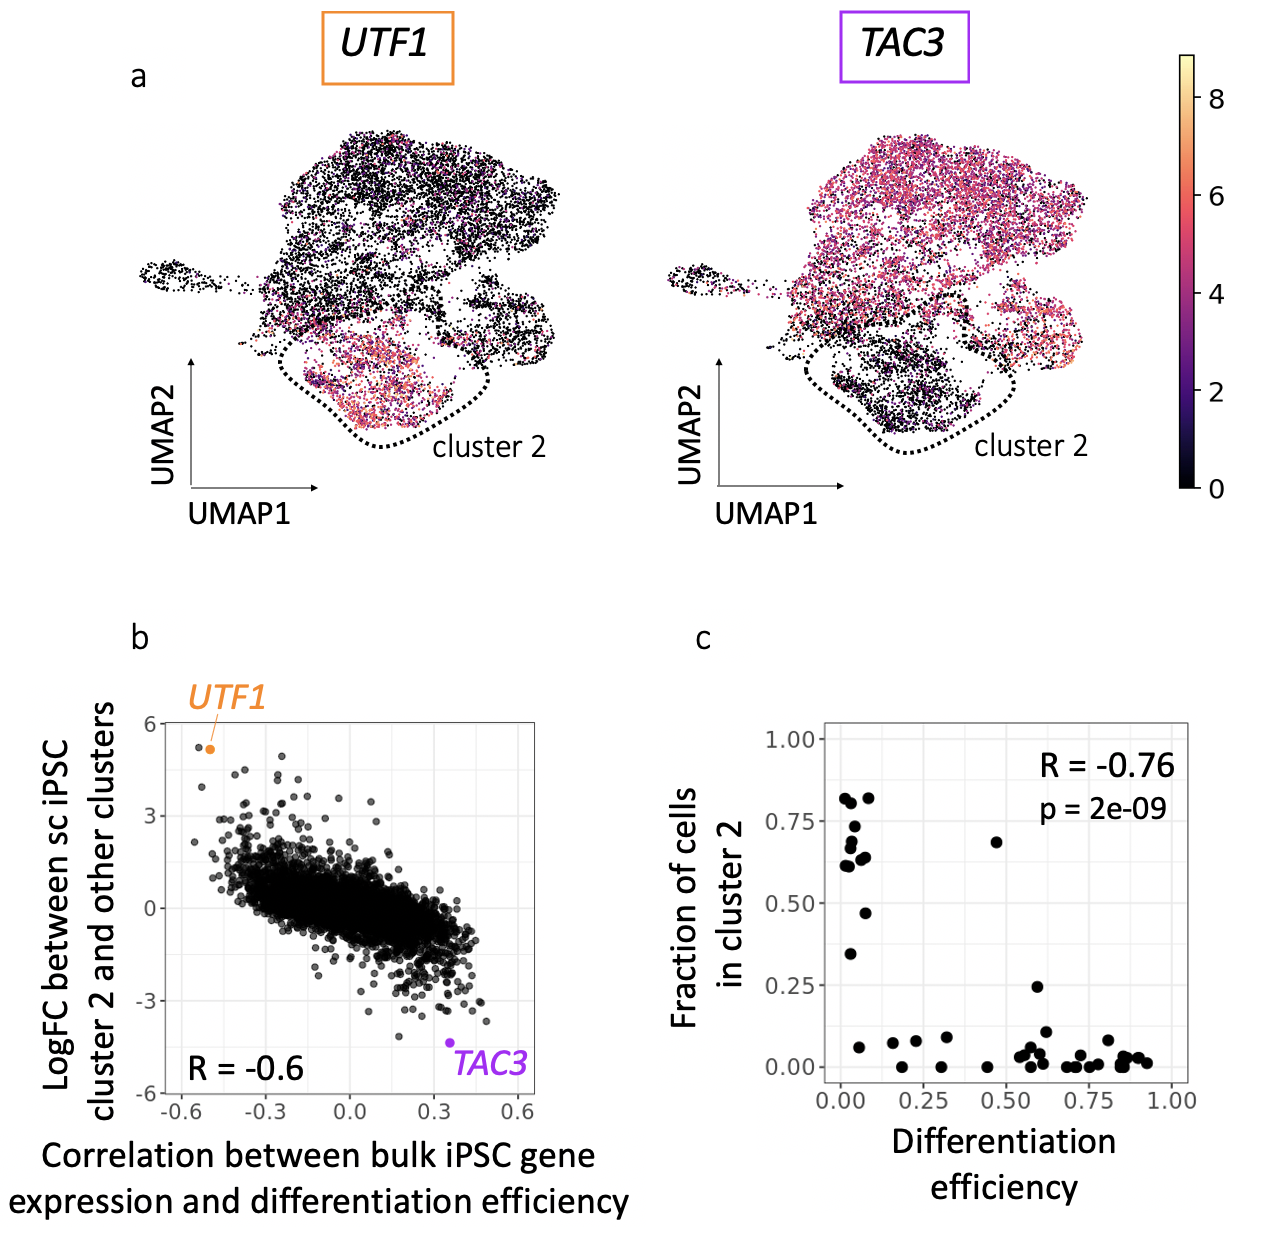
\includegraphics[width=14cm]{Chapter5/Fig/neuroseq_ips_sc_genes.png}
\caption[An iPSC subpopulation is linked to poor differentiation]{\textbf{A subpopulation of iPSCs is associated with poor differentiation}.\\
(a) UMAPs of single-cell RNA-seq profiles in iPSCs from 112 donors \cite{cuomo2020single}.
Colours denote the expression level of the two example genes from \textbf{Fig. \ref{fig:neuroseq_ips_expression_signature}}: \textit{UTF1} and \textit{TAC3}. 
Cluster 2 is shown by the dashed lines. 
(b) Comparison of marker gene association results with expression markers of the cluster 2. 
For each gene, the Pearson correlation coefficient of association between the gene's iPSC expression and neuronal differentiation efficiency (x-axis; iPSC gene expression assessed using bulk RNA-seq, as in \textbf{Fig. \ref{fig:neuroseq_ips_expression_signature}}) is compared to its log fold change between cluster 2 and all other clusters (y-axis, scRNA-seq).
\textit{UTF1}, and \textit{TAC3} are highlighted. 
(c) Scatter plot between the proportion of cells assigned to cluster 2 (y-axis) and neuronal differentiation efficiency (x-axis) across 45 cell lines which were included in both sets of experiments. 
Where measurements across multiple pools were available for a cell line, these were averaged.}
\label{fig:neuroseq_ips_sc_genes}
\end{figure}

Finally, we also analysed an additional scRNA-seq dataset from iPSCs derived from Lymphoblastoid Cell Lines (LCLs) \cite{sarkar2019discovery}. 
Using our single cell analysis pipeline, we identified a cluster of cells with a concordant ($R^2$=0.4) expression profile to cluster 2 (\textbf{Fig. \ref{suppl_fig:ipsc_cluster2_sarkar}}). 
Combined, these results provide further evidence that an iPSC sub-population with poor differentiation capability can be consistently detected across iPSCs from different banks, and that this bias can be predicted robustly using gene expression at iPSC stage. \\

Importantly, despite the variability in neuronal differentiation efficiencies, 
we still retained significant numbers of cells across many cell lines and disease-relevant cell types and stimuli, which 
% our single-cell sequencing approach still 
enabled us to 
% examine multiple disease-relevant cell populations for many cell lines - thus allowing the exploration of 
explore the impact of common genetic variants on gene expression, across such cell populations (next section, \textbf{section \ref{sec:neuroseq_eqt}}).
% these cell types. 
% Correlating changes in gene expression with common genetic variants associated with various traits in GWAS could provide insights into disease mechanisms.

% JCM: Were poorly differentiating lines excluded from subsequent analyses? Could be a little clearer about what's going on here

\newpage

\section{Mapping eQTL in neuronal cell types}
\label{sec:neuroseq_eqt}

Next, in order to understand how individual-to-individual genetic variation influenced gene expression in this system, we mapped \glspl{eqtl} across our identified cell types during differentiation, and in response to stimulation.
Specifically, we mapped \textit{cis} \gls{eqtl} in each of the well represented\footnote{top 4 cell types per condition with at least 20\% cells.} `cell type'-`condition' contexts defined above
% .
% We mapped \gls{eqtl} independently for each of 
i.e.
the 14 distinct cell populations shown in \textbf{Table \ref{tab:eqtl_maps}}. 

\begin{table}[h]
    \centering
    \begin{tabular}{c|c c c c c c}
    &         FPP & P\_FPP & DA & Sert & Epen1 & Astro \\
    \hline
    Day 11  &  \checkmark & \checkmark   \\
    Day 30  & \checkmark & & \checkmark & \checkmark & \checkmark  \\
    Day 52 - untreated & & & \checkmark & \checkmark & \checkmark & \checkmark \\
    Day 52 - ROT treated & & & \checkmark & \checkmark & \checkmark & \checkmark \\
    \end{tabular}
    \caption{Overview of the 14 cell populations we mapped eQTL for.}
    \label{tab:eqtl_maps}
\end{table}

\textit{Cis} \gls{eqtl} were mapped by calculating aggregate expression levels for each donor\footnote{Similar to the total mean aggregation method described in \textbf{Chapter \ref{chapter3}}.}, considering common gene-proximal variants (MAF > 0.05, plus or minus 250 kb around genes). 
For
each context (cell type, condition), all genes detected in at least 1\% of cells of that context
were tested, and expression quantification was only included for a donor if it represented
the mean of at least 10 cells.
The observed variability in neuronal differentiation efficiency between lines\footnote{i.e. as we have seen, some lines made mostly neuronal cell types and barely any non-neuronal, thus expression estimates for those lines in non-neuronal cell types will be less accurate because they are estimated using very few cells, and vice versa for lines that mostly made non-neurons, and very few neurons.} (\textbf{Fig. \ref{fig:neuroseq_diff_efficiency}}) resulted in substantial differences in the number of cells collected for each donor, affecting accuracy of the estimates of aggregated expression. 
To account for this source of noise, we adapted commonly used \gls{eqtl} mapping strategies \cite{cuomo2020single} based on \glspl{lmm} (\textbf{Chapter
\ref{chapter2}})
% 2})
by incorporating an additional variance component into the model:

\begin{equation}\label{eq:neuroseq_ncell}
    \mathbf{y} = \sum_i^{15}\alpha_i \mathbf{PC}_i + \mathbf{g}\beta + \tilde{\mathbf{u}} + \boldsymbol{\psi}, 
\end{equation}

where $\tilde{\mathbf{u}} \sim \mathcal{N}(\mathbf{0}, diag(\frac{1}{n_i}))$, where $n_i$ is the number of cells for each individual i.
% \\
Note that since our LMM implementation only allows one random effect component to be considered (see\textbf{ page \pageref{sec:non_gaussian}}), in this model we are not accounting for population structure.
% JCM: perhaps explain why you are not doing this? Might strike a reader as odd given what you've written in the Introduction chapters?
Consequently, we have to rely on samples being unrelated, and cannot consider multiple observations for the same lines (e.g. across pools). 
Therefore, expression was aggregated at the cell line (and therefore donor) level, averaged across pools for the lines assessed in more than one pool. 

\newpage

% resulting in
Using this approach, we found
a total of 4,828 genes with at least one \gls{eqtl} in any of the contexts (hereafter `eGenes', FDR < 5\%, Storey procedure, \textbf{Table \ref{tab:eqtl_results}}).

\begin{table}[h]
    \centering
    \begin{tabular}{c|c c c c c c}
    &         FPP & P\_FPP & DA & Sert & Epen1 & Astro \\
    \hline
    Day 11  & 2,560 & 2,457 & - & - & - & - \\
    Day 30  & 881 & - &  872 & 776 & 1,011 & -  \\
    Day 52 - untreated & - & - & 1,024 & 1,436 & 1,391 & 257 \\
    Day 52 - ROT treated & - & -  & 458 & 1,043 & 1,122 & 205 \\
    \end{tabular}
    \caption{Number of eGenes at FDR < 5\% for each assessed eQTL map.}
    \label{tab:eqtl_results}
\end{table}


This approach greatly increased the power to map \gls{eqtl},
% Power is greatly increased 
as compared to the base-model which does not include the noise term, i.e.:

\begin{equation}\label{eq:neuroseq_base}
    \mathbf{y} = \sum_i^{15}\alpha_i \mathbf{PC}_i + \mathbf{g}\beta + \boldsymbol{\psi},
\end{equation}
% Power is greatly increased compared to the base-model which does not include the noise term, i.e.:

confirming the importance of taking into account, in the model, the large effect that the number of cells for each individual has on the 
uncertainty
% accuracy 
of the mean expression estimation (\textbf{Fig. \ref{fig:neuroseq_eqtl_improved_power}}).


% Base:            y = PC1:15 + SNP + noise
% Our model:   y = PC1:15 + SNP + 1/n + noise

\begin{figure}[h]
\centering
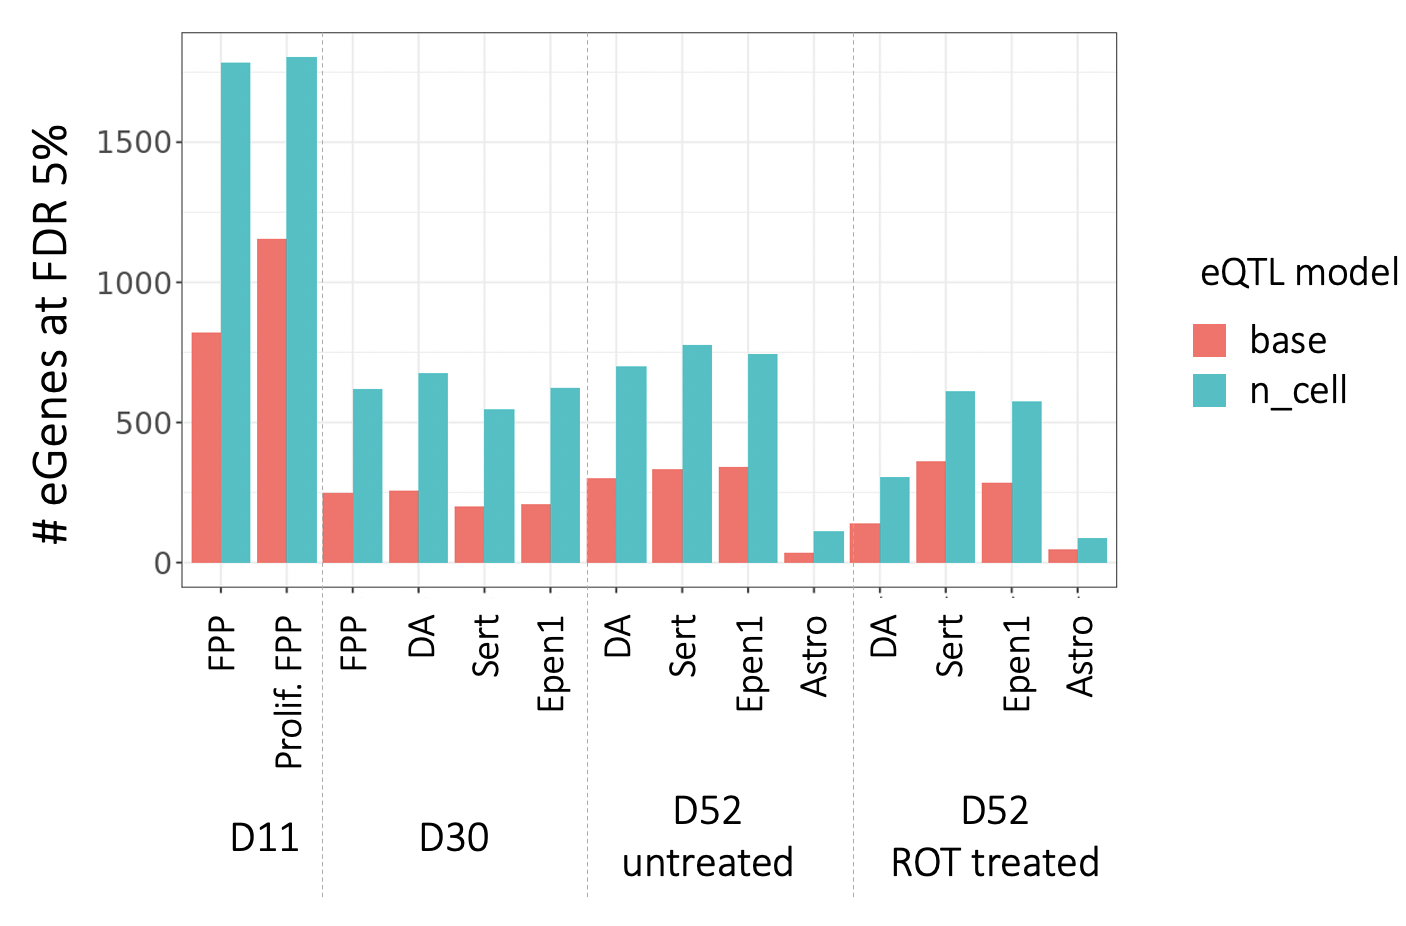
\includegraphics[width=13cm]{Chapter5/Fig/neuroseq_eqtl_power.png}
\caption[Improved eQTL power]{\textbf{Improved eQTL power}.\\
Number of eGenes for each cell type, time point and stimulation discovered using either a traditional linear model (coral, from eq. \eqref{eq:neuroseq_base}) or our enhanced model accounting for noise due to variation in the number of cells collected for each donor (seagreen, from eq. \eqref{eq:neuroseq_ncell}).}
\label{fig:neuroseq_eqtl_improved_power}
\end{figure}


\subsection{Comparison with alternative eQTL methods}

For one exemplar eQTL map (untreated dopaminergic neurons at day 52), we also compared our results (which yelded 1,024 eGenes, \textbf{Table \ref{tab:eqtl_results}}) to those obtained from alternative eQTL methods, demonstrating that our results are robust to these specific choices, with the strategy we chose yielding more total eQTL discoveries. 
In particular, by aggregating at the donor level, we may not be accounting properly for batch differences.
As an alternative, we could aggregate at the line and experiment level (similar to the approach described in \textbf{Chapter 
% 4
\ref{chapter4}}), and use a standard kinship matrix-approach to account for the repeatedness (rather than the number of cells noise term), i.e test the following model:

% Model 0: y = PC1:15 + SNP + K + noise (471 eGenes).
\begin{equation}\label{eq:neuroseq_pcs_kinship}
    \mathbf{y} = \sum_i^{15}\alpha_i \mathbf{PC}_i + \mathbf{g}\beta + \mathbf{u} + \boldsymbol{\psi}, 
\end{equation}
where $ \mathbf{u} \sim \mathcal{N}(\mathbf{0},\sigma_g^2\mathbf{K})$;
this resulted in 471 eGenes at FDR < 5\%.\\

Another possibility would be to include the batch directly as (several) covariates, 
% and then attempt to account for the number of cells per individual as a fixed effect term, 
such that:

% Model 2: y = pool + SNP + K + noise (320 eGenes).
\begin{equation}\label{eq:neuroseq_batch_kinship}
    \mathbf{y} = \sum_i^{16}\alpha_i \mathbf{pool}_i + 
    % \gamma \ \mathbf{n} + 
    \mathbf{g}\beta + \mathbf{u} + \boldsymbol{\psi}, 
\end{equation}

where $ \mathbf{u} \sim \mathcal{N}(\mathbf{0},\sigma_g^2\mathbf{K})$.
% and $\mathbf{n}$ is the vector of $n_i$. 
This resulted in markedly fewer eGenes - 320.\\

Finally, in order to account for batch effects whilst still including the number-of-cell noise term, it is possible to only consider one experiment per line, and correct for pool, as well as sex, as covariates:
% Model 1: y = pool + sex + SNP + 1/n + noise  (identifies 398 eGenes)
\begin{equation}\label{eq:neuroseq_batch_ncell}
    \mathbf{y} = \sum_i^{16}\alpha_i \mathbf{pool}_i + \gamma \ \mathbf{sex} + \mathbf{g}\beta + \tilde{\mathbf{u}} + \boldsymbol{\psi}, 
\end{equation}

where $\tilde{\mathbf{u}} \sim \mathcal{N}(\mathbf{0}, diag(\frac{1}{n_i}))$, and $n_i$ is the number of cells for each individual i, as above.
This approach, too, resulted in fewer eGenes, 608.\\

Overall, our approach was the best powered (with 1,024 eGenes, see \textbf{Table \ref{tab:eqtl_results}}), yet the results were highly consistent between methods (\textbf{Fig. \ref{fig:neuroseq_eqtl_methods_comp}}), excluding the possibility that our model may be generating mainly false positives.

\begin{figure}[htbp]
\centering
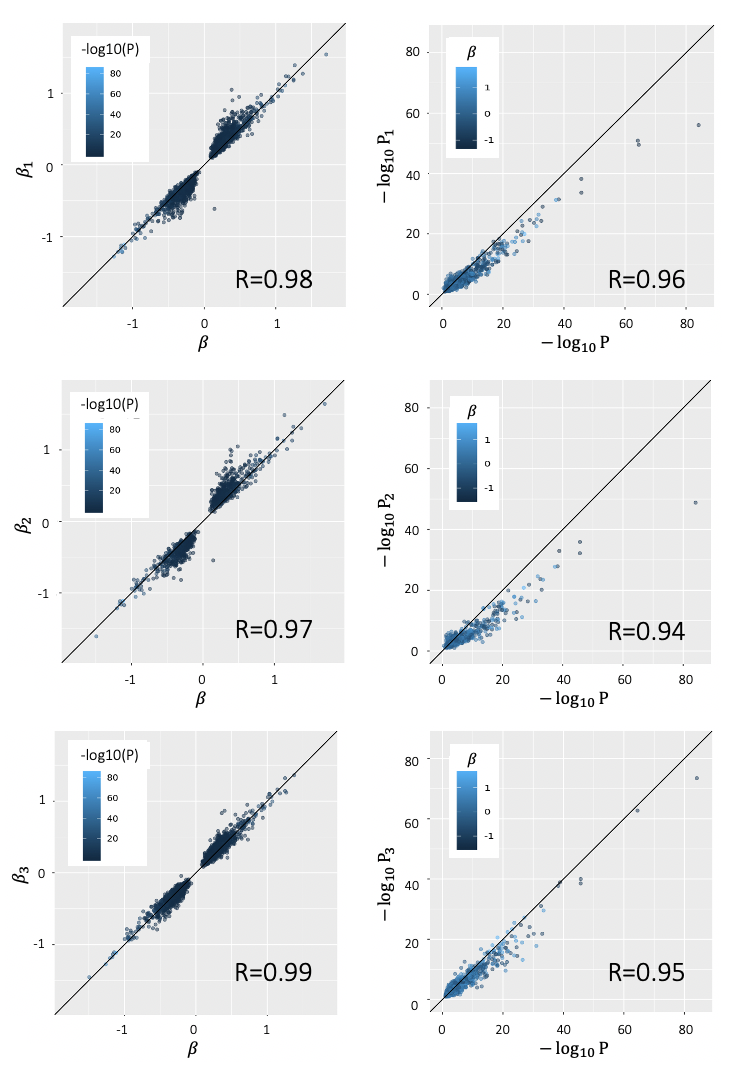
\includegraphics[width=13.5cm]{Chapter5/Fig/neuroseq_eqtl_methods_corr.png}
\caption[eQTL methods comparison]{\textbf{eQTL methods comparison}.\\
Scatter plots of \gls{eqtl} effect sizes (left) and p values (right) obtained when testing association of untreated day 52 dopaminergic neuron \gls{eqtl} discovered using our approach (from eq. \eqref{eq:neuroseq_ncell}, x axis) and each of the three alternative methods described in equations \eqref{eq:neuroseq_pcs_kinship}, \eqref{eq:neuroseq_batch_kinship} and \eqref{eq:neuroseq_batch_ncell}, respectively (y axis). 
Pearson's correlations (R) are indicated.}
\label{fig:neuroseq_eqtl_methods_comp}
\end{figure}

% % Our approach also improved power compared to other model tried to address reviewers..

% % Having said this, we now present results obtained from alternative eQTL methods for 
% For 
% one exemplar eQTL map (untreated dopaminergic neurons at day 52), we also compared our results to those obtained from alternative eQTL methods, demonstrating that our results are robust to these specific choices with the strategy we present in the main text yielding more total eQTL discoveries. 

% As mentioned above,
% % In particular, we note that
% in the current model expression level $\mathbf{y}$ is aggregated at the donor/line level, therefore it is aggregated across pools in the case of a line differentiated in multiple pools. 
% As such, 
% we could not directly correct for batch effects, as
% adding the pool as a covariate would be ill-defined. \\

% To circumvent this issue, it is possible to i) only select one pool for each line, ii) include both replicates per line across pools. 
% In the second case, samples are not genetically independent, and we need to account for the replicated structure using the random effect term.
% For reference the model used for the results presented in the main text identified 698 eGenes for DA D52 NONE.

% Model 1 uses the first approach of selecting only one pool per line. In addition, we account for pool effects as well as effects of donor sex as covariates:


% Model 1: y = pool + sex + SNP + 1/n + noise  (identifies 398 eGenes)

% % Model 1b is equivalent but we also add age as a covariate (limited to 153/175 lines for which we have age information):

% % Model 1b: y = pool + sex + age + SNP + 1/n + noise (identifies 209 eGenes)

% Model 2 uses the second approach and include n (number of cells per donor, pool) as a covariate.

% Model 2: y = pool + n + SNP + K + noise (213 eGenes).

% \subsubsection{PCs}

% Moreover, the inclusion of PCs to capture global trends in expression is fairly standard in eQTL mapping studies (cite GTEx, and many others). In general, PCs do capture global trends and hence “subsume” common technical covariates.
% Finally, to assess whether the PCs do indeed  capture the key known covariates, we fitted a linear model for different covariates as a function of the 15 PCs used as covariates i.e.:

% Covariate (e.g. sex) = PC1 + ... + PC15 + noise

% and found the following: the 15 PCs explained 67\% of the variance of the donor sex covariate (male=0, female=1), 9\% of average age (age is provided as a categorical variable, we take the mid value and treat it as numeric, e.g. [40-44] becomes 42).

\clearpage

\subsection{Comparison of eQTL across cell types and conditions}

% Now that the validity of our results was established,
Next, we set out to compare eQTL maps across cell types and conditions.
First, we observed that the largest number of \gls{eqtl} were detected in progenitor cell populations, likely reflecting increased detection power due to the larger number of well-represented donors (> 100 cells per donor). 
Next, we noted that the cumulative number of eGenes (genes with an \gls{eqtl}) in each cell type increased considerably when taking into account cells further progressed along the differentiation axis, as well as upon stimulation (\textbf{Fig. \ref{fig:neuroseq_eqtl}}). 


\begin{figure}[h]
\centering
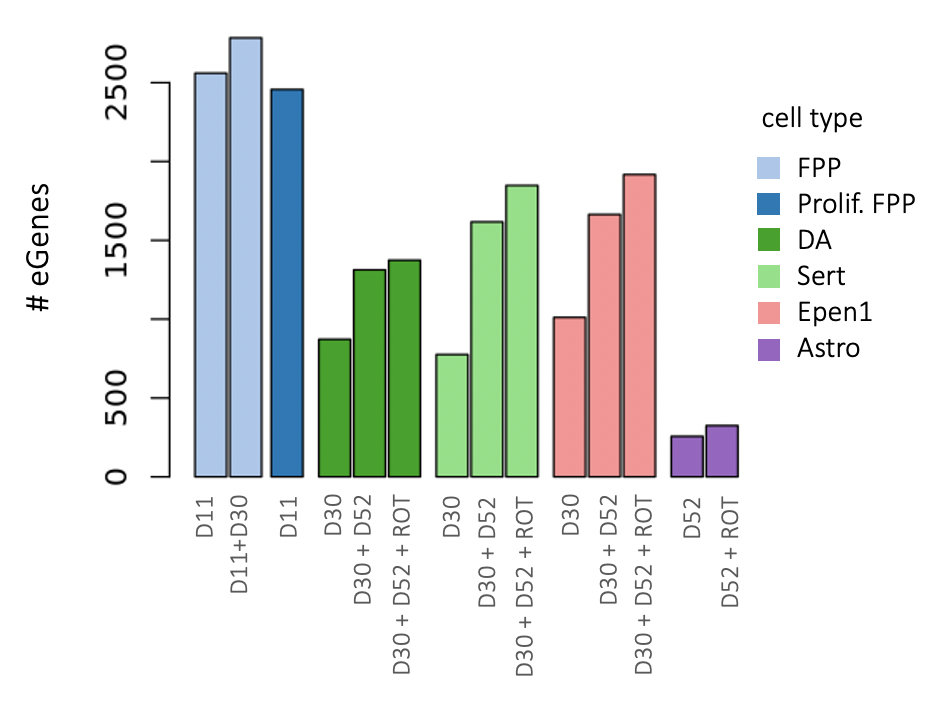
\includegraphics[width=14cm]{Chapter5/Fig/neuroseq_eqtl_cumulative.png}
\caption[Mapping eQTL across neuronal cell types]{\textbf{Mapping \textit{cis} eQTL in distinct cell contexts across midbrain differentiation}.\\
% (a)Number of genes with at least one eQTL (eGenes) for each cell type and condition.
% (b)
Cumulative number of eGenes for each cell type and condition (D11 = day 11; D30 = day 30; D52 = day 52 (untreated); ROT = rotenone-treated day 52).}
\label{fig:neuroseq_eqtl}
\end{figure}

For example, in DA cells, eQTL mapping in matured (untreated) cells (day 52) identified an additional set of 441 eGenes (at FDR < 5\%) compared to day 30 cells.
An example of a timepoint-specific eGene is \textit{HSPB1}, for which SNP rs6465098 is an eQTL in day 52 cells, but not day 30 (\textbf{Fig. \ref{fig:neuroseq_eqtl_examples}}). 
\textit{HSPB1} encodes a heat shock protein that plays a key role in neuronal differentiation \cite{miller2018heat} and for which changes in gene expression have been observed in neurons after ischemia \cite{bartelt2016hspb5} and associated with toxic protein accumulation in Alzheimer's disease \cite{shimura2004binding, wilhelmus2006small}.\\

Similarly, we detected 248 additional eGenes with a rotenone-specific effect in DA and Sert neurons. 
As an example, the SNP variant rs12597281 is an eQTL for \textit{ACSF3} in rotenone-stimulated serotonergic-like neurons at day 52, but not in unstimulated cells (\textbf{Fig. \ref{fig:neuroseq_eqtl_examples}}). 
\textit{ACSF3} encodes an acyl-CoA synthetase localised in the mitochondria and for which inherited mutations have been associated with a metabolic disorder, combined malonic and methylmalonic aciduria (CMAMMA), where patients exhibits a wide range of neurological symptoms including memory problems, psychiatric problems and/or cognitive decline \cite{tucci2020brain}.\\

These examples highlight how changes in the expression of genes known to be associated with human disease can be transient and specific to a cell type and state. 
More importantly, this data shows how our experimental design brings an extra level of resolution to understand disease mechanisms that were previously inaccessible from primary tissues, and opens up new experimental avenues. \\


% \begin{figure}[h]
% \centering
% 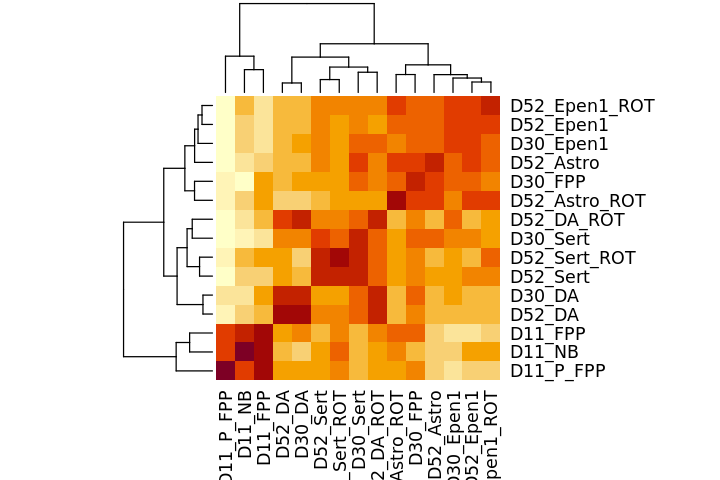
\includegraphics[width=16cm]{Chapter5/Fig/neuroseq_eqtl_neuroseq_heatmap.png}
% \caption[Sharing of eQTL withing study]{\textbf{Sharing of eQTL withing study}.\\
% .}
% \label{fig:neuroseq_eqtl_heatmap}
% \end{figure}

\begin{figure}[h]
% \centering
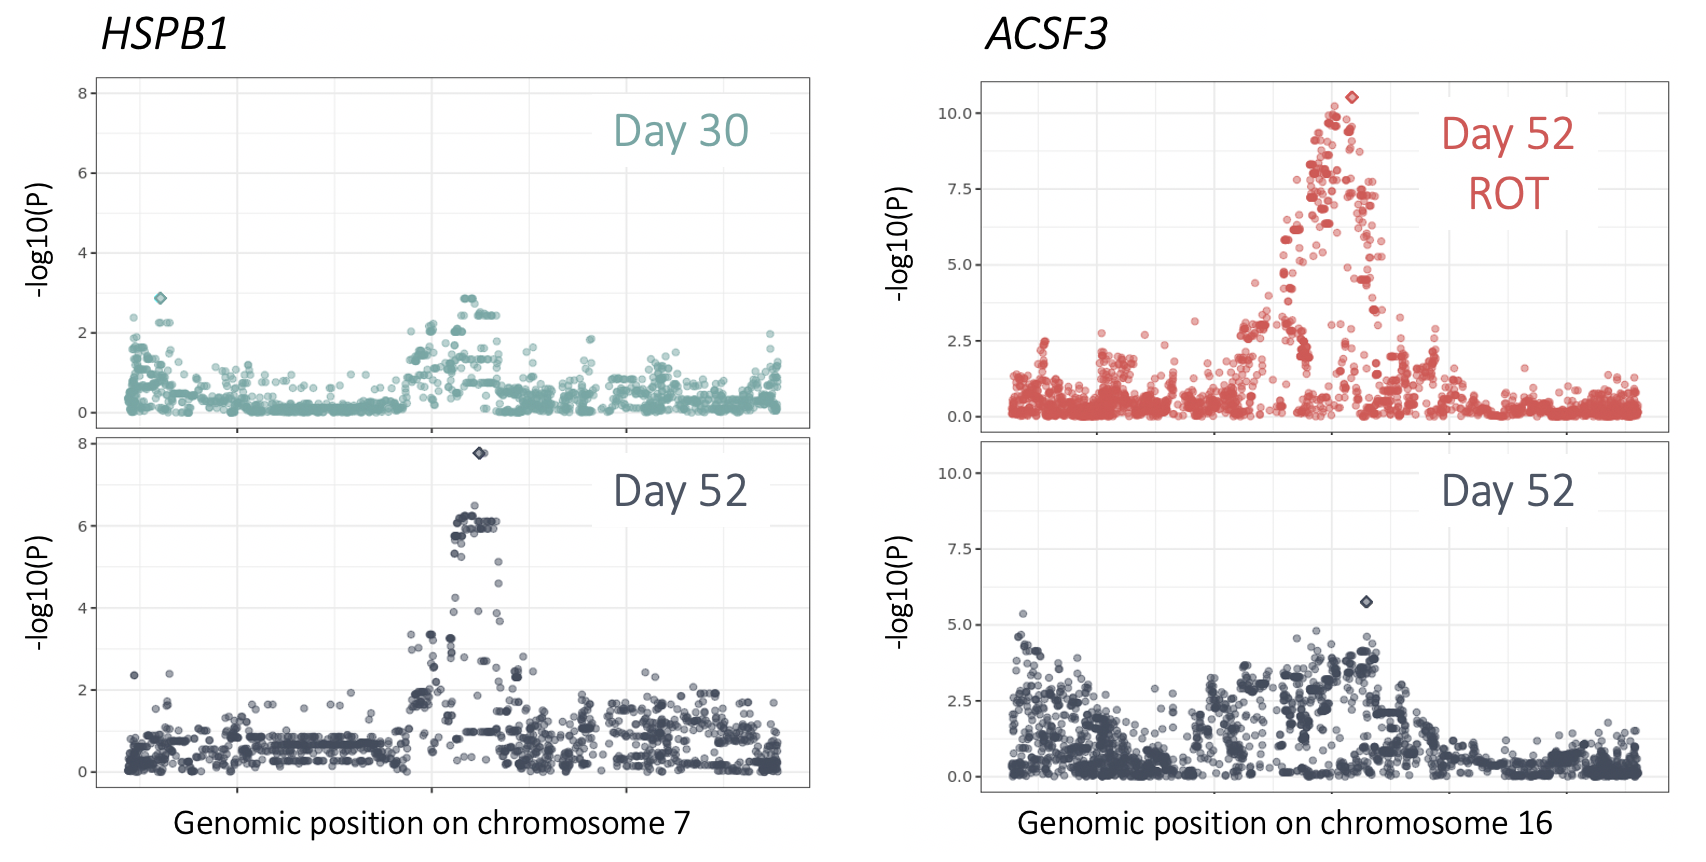
\includegraphics[width=16cm]{Chapter5/Fig/neuroseq_eqtl_examples.png}
\caption[Context-specific eQTL examples]{\textbf{Context-specific eQTL examples}.\\
Left: day 52-specific eQTL for \textit{HSPB1} in DA (rs6465098; FDR < 5\%). 
In figure are Manhattan plots for DA cells at day 30 (top) and day 52 (bottom). 
Right: a rotenone stimulus-specific eQTL for \textit{ACSF3} in serotonergic-like neuronal cells (rs12597281, right). 
Manhattan plots are shown for rotenone-stimulated (top) and unstimulated (bottom) Sert day 52 cells.}
\label{fig:neuroseq_eqtl_examples}
\end{figure}

\clearpage

\subsection{Comparison of eQTL from our study with \textit{in vivo} maps}

In order to put our eGene discovery in relation to previous studies, we compared the number of eGenes identified here with bulk eQTL maps from \textit{in vivo} tissues from the GTEx consortium \cite{gtex2017genetic}. 
% To aid the comparison 
For a first coarse-grain comparison between bulk and single-cell eQTL maps,
we aggregated\footnote{Considered the union of eQTL identified in any of our 14 cell populations.} eQTL across cell types and found that the number of discovered eGenes was similar to that expected in a primary tissue of the same sample size (\textbf{Fig. \ref{fig:neuroseq_and_gtex_power}}). \\

However, when focusing on individual cell populations, we observed fewer `cell type'-`condition' eGenes than detected in GTEx tissues of similar sample size (\textbf{Fig. \ref{fig:neuroseq_and_gtex_power}}), likely due to the uneven representation of donors across cells, which in turn results in noisier expression estimates compared to the GTEx results using bulk measurements.
This result is consistent with what we observed in work presented in \textbf{Chapter \ref{chapter3}}, where we found increased power when mapping eQTL using bulk compared to single cell RNA-seq, even when considering the same cell type and matched individuals. 
% \\

% JCM: Because of noise in the estimate? Less noise in the GTEX measurement? Could interpret this better for the reader I think. It's a little bit too cryptic at present I think.
\vspace{2mm}

\begin{figure}[h]
% \centering
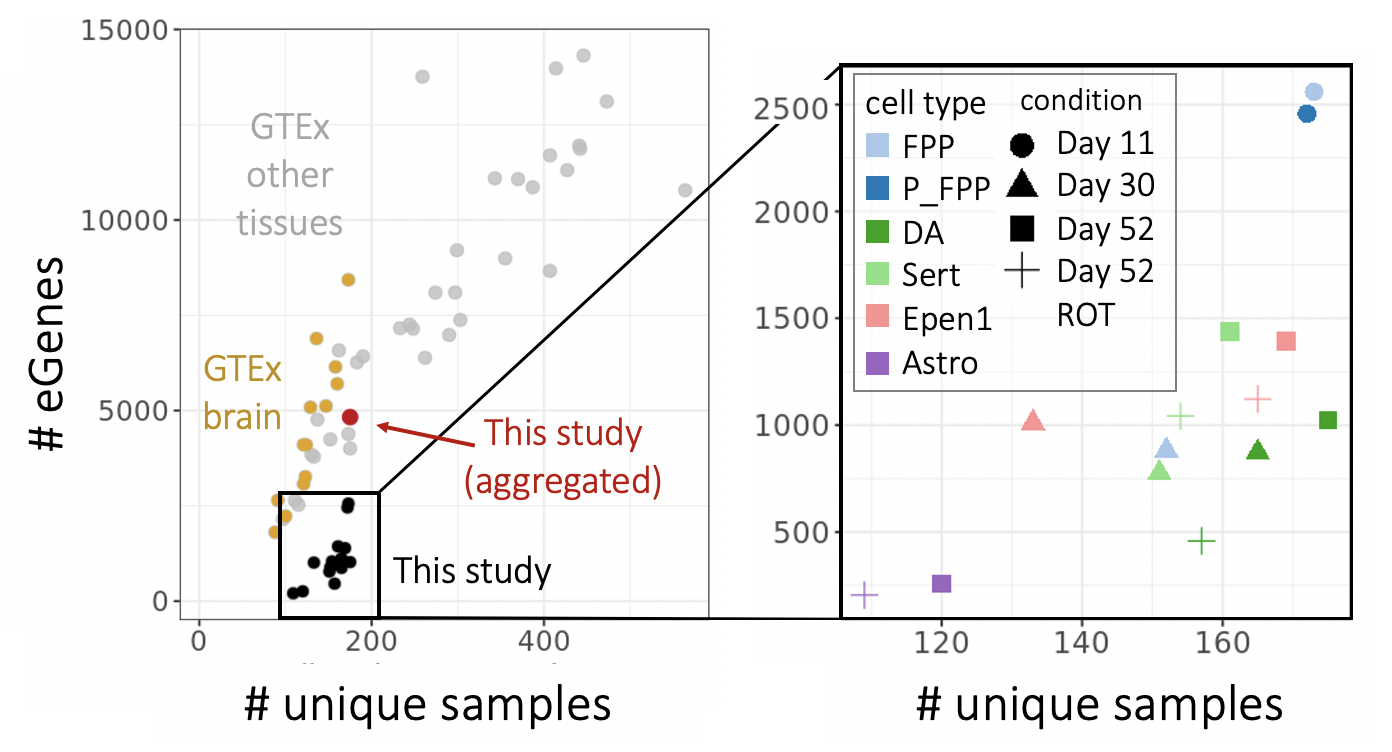
\includegraphics[width=15cm]{Chapter5/Fig/neuroseq_eqtl_gtex_scatterplot.png}
\caption[Sample size vs power]{\textbf{Sample size vs power}.\\
Comparison of the number of genes with at least one eQTL (number of eGenes; FDR < 5\%; y-axis) as a function of effective sample size (number of unique donors; x-axis) across studies and cell types. 
Left: results from overlapping eQTL results in this study with \textit{in vivo} eQTL maps from GTEx, divided into brain tissues and non-brain tissues. 
The result from our study when aggregating across cell types and conditions is coloured in red. 
The right panel shows a magnified view of results from our study coloured by cell type and shaped by condition.}
\label{fig:neuroseq_and_gtex_power}
\end{figure}

\newpage

% JCM: Introduce this a little better? 'Next, we explored a key question: do our eQTL maps from in vitro models resemble eQTL maps from equivalent in vivo systems?' or something like that...

A key question of eQTL maps from \textit{in vitro} iPSC-based models is how closely these resemble eQTL maps from the equivalent primary tissues, which typically differ in cell type composition. \\ 

To explore this, we tested the extent to which regulatory variants were shared between our eQTL maps and 48 
% (?)
\textit{in vivo} maps from the GTEx consortium, 
% in three resources: 1) the current study, 2) GTEx brain tissues (n=13 tissues), and 3) bulk and single-cell RNA-seq profiles of HipSci iPS cell lines \cite{bonder2019systematic, cuomo2020single}, 
as measured by genome-wide consistency of eQTL effect sizes (using MASHR \cite{urbut2019flexible}).
% Briefly, .. maybe add MASHR details here?
First, reassuringly, we observed that the sharing of genetic signal\footnote{Following recommendations by the MASHR authors \cite{stephens2020eqtl}, for each pair of conditions, we considered eQTL that were significant (local false sign rate < 0.05) in at least one of the two conditions, and then assessed sharing as the fraction of those for which posterior estimates of effect size were of similar magnitude ($0.5 <$ ratio $<2$) and of concordant direction of effect.} between our eQTL maps and GTEx tissues is consistently higher when we consider brain tissues compared to all other tissues (\textbf{Fig. \ref{fig:neuroseq_and_gtex_brain_specificity}}, using the subset of 6,205 genes that were assessed in each of our cell types and in all GTEx tissues). 
% The number of genes tested here is 6,205.
\\

\begin{figure}[h]
\centering
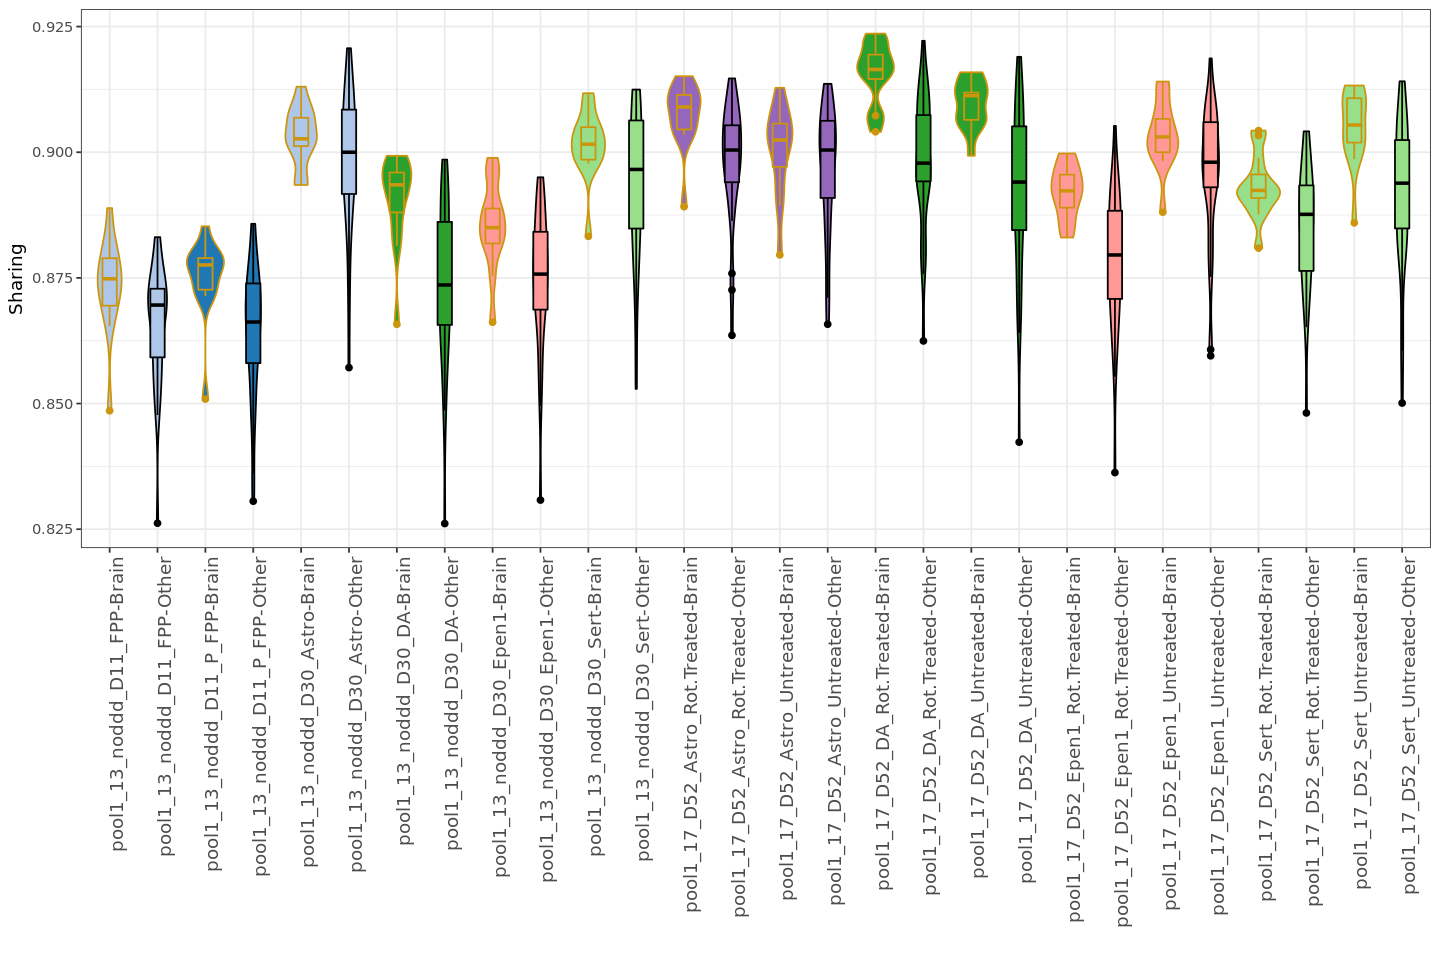
\includegraphics[width=16cm]{Chapter5/Fig/neuroseq_gtex_brain_nonbrain_boxplots.png}
\caption[Brain vs non-brain]{\textbf{Brain vs non-brain - rearrange box plot, update to new results}.\\
Box plots indicating for each of our 14 eQTL maps (on the x axis) the amount of sharing as quantified by MASHR \cite{urbut2019flexible} with each of the GTEx brain tissues (yellow, n=13) and GTEx other (non-brain) tissues (black, n=36).
Box plots are coloured by cell type, whereas the border indicates the set of GTEx tissues considered.}
\label{fig:neuroseq_and_gtex_brain_specificity}
\end{figure}

\newpage

Next, we performed a second MASHR analysis, this time including only the 13 GTEx brain tissues (as well as our 14 maps).
The main motivation to do so is that in order to quantify the amount of sharing between eQTL results obtained from several tissues or conditions, MASHR only considers gene-SNP pairs that have been assessed in every one of the conditions considered, which naturally will depend on the number of genes expressed in the various conditions and that can be quantified by the different technologies used. 
% It can only do so for 
% genes that are expressed enough to be assayed across all conditions.
\\

As a consequence, the number of genes considered decreases as the number of conditions included increases, which in turn results in the inflation of the amount of sharing.
% \\
Here, in particular, excluding non-brain eQTL maps from GTEx rescued several brain-specific genes, and allowed us to assess sharing for 8,706 genes ($\sim$2,500 more).
This second analysis enabled us to assess the similarity of our maps to the brain tissues in particular (\textbf{Fig. \ref{fig:neuroseq_and_gtex_brain_sharing}}). \\

\begin{figure}[h]
\centering
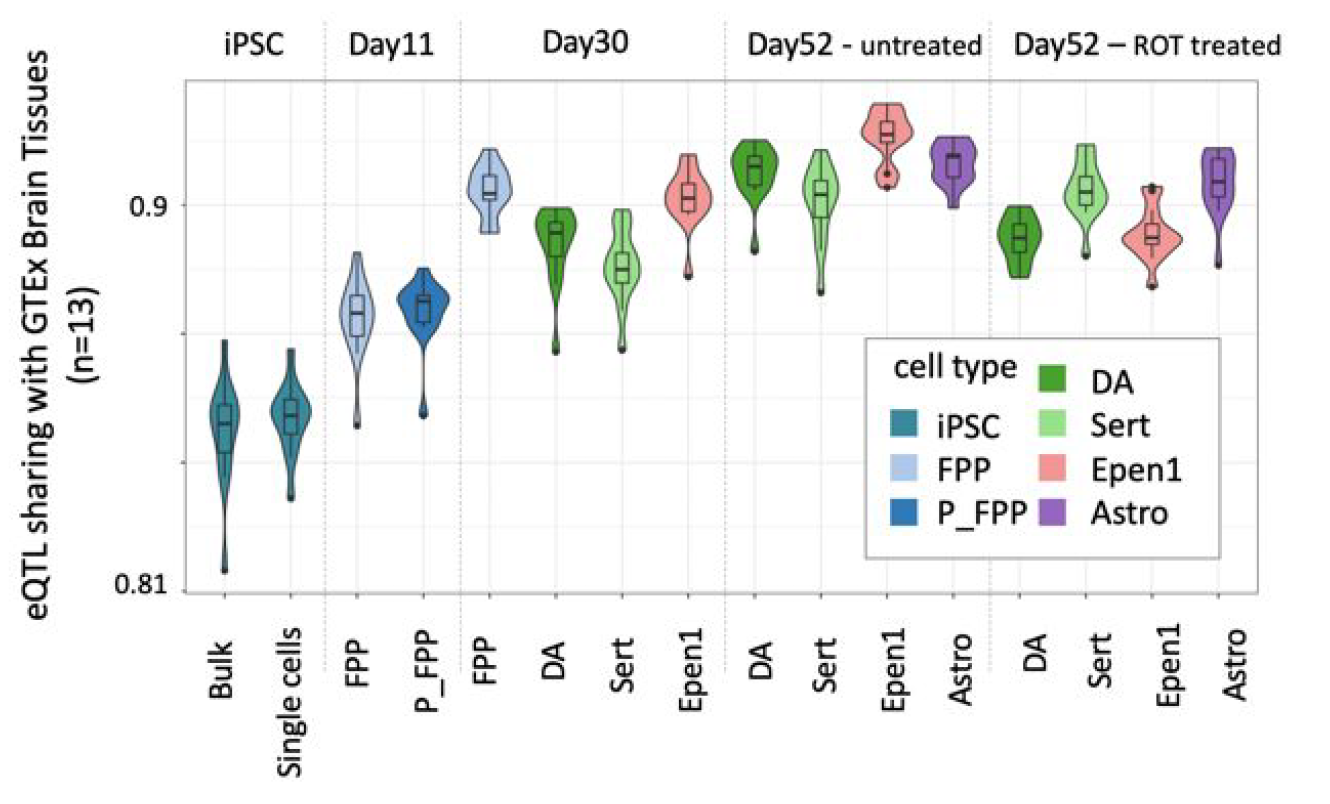
\includegraphics[width=16cm]{Chapter5/Fig/neuroseq_gtex_brain_boxplots.png}
\caption[Brain sharing increase]{\textbf{Brain sharing increases over time}.\\
Sharing of eQTL signals discovered in our study for different cell types and conditions, 
% as well as in two recent iPSC studies \cite{cuomo2020single, bonder2019systematic} 
with \textit{in vivo} brain eQTL maps (from GTEx). 
Violin plots show the extent of eQTL sharing with each of 13 GTEx brain eQTL maps.
% For reference, sharing between one of the GTEx brain tissue (the substantia nigra) and the others (excluding itself, n=12).
}
\label{fig:neuroseq_and_gtex_brain_sharing}
\end{figure}

% For reference, we included the similarity with brain maps for two selected GTEx brain tissues (Fig. \ref{fig:neuroseq_and_gtex_brain_sharing}). 
% This is similar to what is shown in Figure 4D, but this time we are including genes that are expressed in brain and in our data (without requesting that they should be expressed in e.g. liver, or heart). 
We found that the extent of eQTL sharing between our eQTL maps and GTEx brain tissues increased as iPSCs were differentiated to increasingly mature neuronal cell types (\textbf{Fig. \ref{fig:neuroseq_and_gtex_brain_sharing}}). \\

This result provides confidence that eQTL discovered in iPSC-derived neuronal cell types mimic eQTL maps from \textit{in vivo} tissues. 
Consistent with the trend of increased sharing of eQTL signal, we also observed that the fraction of eQTL that are not represented in GTEx brain tissues decreases as the cells become increasingly mature. 
In particular, we identified 2,366 eQTL that could not be detected in GTEx brain tissues (q value > 0.05 in any of the 13 tissues), demonstrating the utility of iPSC and scRNA-seq analysis to assess previously unexplored cell populations and therein discover regulatory changes in disease associated genes. \\

Finally, we note that quantifying the amount of sharing of eQTL signal is a notoriously difficult problem.
As mentioned, MASHR considers only genes assessed in all conditions analysed. 
As a result, the degree of sharing may be inflated, because only relatively few highly expressed genes are included in the analysis, and those are more likely to be common eQTL. 
In particular using scRNA-seq we can assay fewer genes (as compared to bulk), thus the number of genes that we can assess in our single cell maps becomes the limiting factor in terms of genes included in the analysis (i.e. 8,706/8,738 genes assessed in all of our maps are also assessed in all GTEx brain maps).\\

% MASHR is probably overestimating the amount of sharing.
% Also, only genes assessed (i.e. expressed) in all conditions are included.\\

On the other hand,
% In contrast, 
we can investigate what portion of eQTL from a GTEx map can be rediscovered in our data.
As exemplar maps, at varying sample sizes, we took the substantia nigra (n=88), the frontal cortex (n=129) and the cerebellum (n=173) GTEx (brain) maps.
% The substantia nigra is also the only midbrain region from the GTEx maps.
% The cerebellum is often an outlier brain tissue, with especially many eQTL (ref).
Of the eGenes identified at FDR < 5\% in each of the GTEx maps, a little bit less than 60\% of the genes were tested in any of our maps 
(985/1,807 (55\%) for substantia nigra,
3,034/5,086 (60\%) for frontal cortex, 
and 5,204/8,429 (62\%) for cerebellum).
For those, 55\% eQTL were nominally significant (p value < 0.05) in at least one of our maps (on average, substantia nigra: 57\%, cerebellum: 59\%, frontal cortex: 49\%), 
% Even more rarely were both the gene and the genetic variant assessed in our maps (from 398 to 420, about 20\%).
% From 197 to 262 of these eQTL (about 60\%) were nominally significant in our maps, most of which
and most of them
(90\% on average) also had consistent effect sign. \\

So in total, around 30\% of the eQTL (29\%, 31\%, 36\%)
from a GTEx brain map could be re-discovered in one of our single cell neuronal maps (\textbf{Fig. \ref{fig:neuroseq_and_gtex_rediscovery}}).

\begin{figure}[h]
\centering
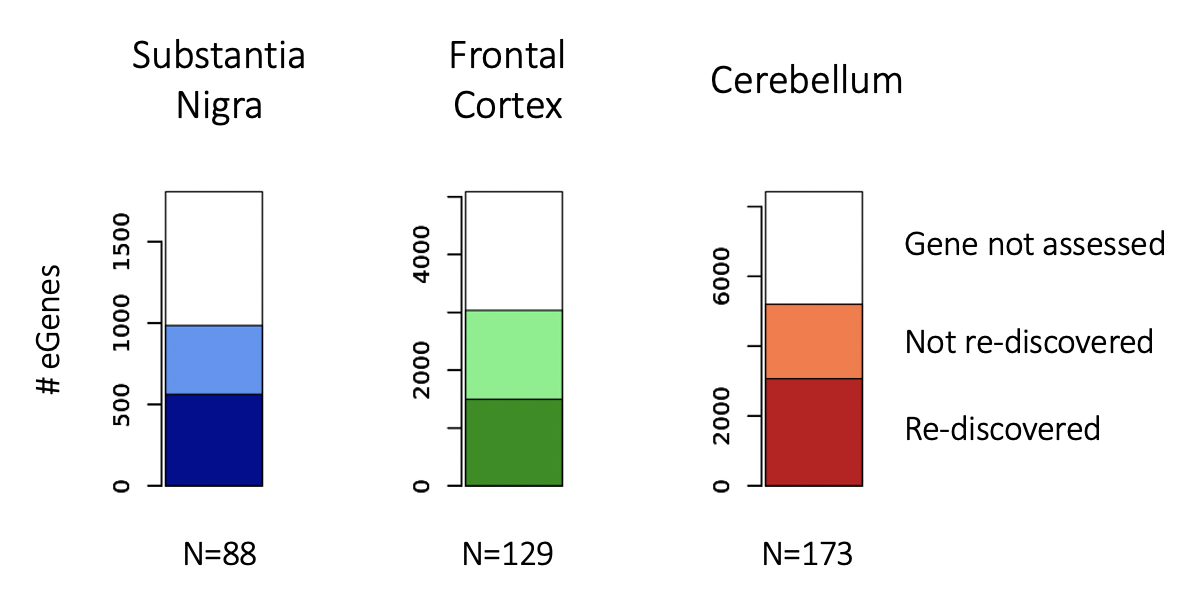
\includegraphics[width=16cm]{Chapter5/Fig/neuroseq_rediscovering_gtex_brain.png}
\caption[Rediscovery of GTEx brain eQTL maps]{\textbf{Rediscovery of GTEx brain eQTL maps}.\\
For three representative GTEx brain tissue-eQTL maps of various sample size (substantia nigra, n=88; frontal cortex, n=129; cerebellum, n=173), we divide eGenes (genes with at least one eQTL, FDR < 5\% in the GTEx eQTL map) into i) genes that were not assessed in any of our maps (white), ii) genes that were assessed in at least one of our maps, but whose lead variant could not be re-discovered (light colour, nominal p value > 0.05 in all of our 14 eQTL maps) and iii) genes whose lead eQTL variant who could be rediscovered (dark colour, nominal p value < 0.05 in at least one of our 14 maps).}
\label{fig:neuroseq_and_gtex_rediscovery}
\end{figure}

% JCM: Perhaps put this in context - at face value it seems like a pretty poor result so some contextualisation here (or at least pointing to the discussion) would be helpful I think.


% MASHR \cite{urbut2019flexible} quantifies the amount of sharing between eQTL results obtained from several tissues or conditions. It can only do so for genes that are expressed enough to be assayed across all conditions considered. As a consequence, the degree of sharing is inflated because only relatively few highly expressed genes are included in the analysis, and those are more frequently shared eQTL.
% We have now performed three sets of analyses, when we run MASHR on i) all of our cell types and conditions (n=14), as well as all of the GTEx tissues (n=49); ii) all of our cell types and conditions (n=14), as well as all of the GTEx brain tissues (n=13) and iii) only our cell types and conditions (n=14), 


% To explore this, we tested the extent to which regulatory variants were shared between eQTL maps in three resources: 1) the current study, 2) GTEx brain tissues (n=13 tissues), and 3) bulk and single-cell RNA-seq profiles of HipSci iPS cell lines \cite{bonder2019systematic, cuomo2020single}, as measured by genome-wide consistency of eQTL effect sizes (using MASHR 42 \cite{urbut2019flexible}). 
% We found that as iPSCs were differentiated to increasingly mature neuronal cell types, the extent of eQTL sharing consistently increased (Fig. \ref{fig:neuroseq_and_gtex_brain_sharing}). 
% This provides additional confidence that eQTL discovered in iPS-derived neuronal populations mimic \textit{in vivo} eQTL maps. 
% Consistent with the trend of increased eQTL sharing, we also observed that the fraction of eQTL that are not represented in GTEx brain tissues decreases as the cells become more mature. 
% Interestingly, while iPS-derived eQTL maps mimic \textit{in vivo} GTEx Brain eQTL maps, we also identified 2,203 eQTL that could not be detected in GTEx brain tissues (q value > 0.05 in any of 13 tissues), demonstrating the utility of iPSC and scRNA analysis to discover regulatory changes in disease associated genes.\\

% MASHR \cite{urbut2019flexible} quantifies the amount of sharing between eQTL results obtained from several tissues or conditions. It can only do so for genes that are expressed enough to be assayed across all conditions considered. As a consequence, the degree of sharing is inflated because only relatively few highly expressed genes are included in the analysis, and those are more frequently shared eQTL.
% We have now performed three sets of analyses, when we run MASHR on i) all of our cell types and conditions (n=14), as well as all of the GTEx tissues (n=49); ii) all of our cell types and conditions (n=14), as well as all of the GTEx brain tissues (n=13) and iii) only our cell types and conditions (n=14), 

% We use the first analysis to show that sharing of genetic signal between our eQTL maps and GTEx tissues is consistently higher when we consider brain tissues compared to all other tissues (Fig. \ref{fig:neuroseq_and_gtex_brain_specificity}). The number of genes tested here is 6,205.


% Finally, the last analysis assesses specifically similarities and differences between our cell types only (8,738 genes used, Fig. \ref{fig:neuroseq_eqtl_heatmap}). 



\clearpage

\section{Colocalisation of eQTL with disease risk variants}
\label{sec:neuroseq_coloc}

The identified cell-type specific eQTL maps across different differentiation contexts provide an exciting opportunity to improve our understanding of human disease traits and their genetic risk factors identified by GWA studies.
To systematically test for colocalisation events (\textbf{page \pageref{sec:eqtl_gwas}}), we applied COLOC \cite{giambartolomei2014bayesian} to the summary statistics from 25 neurological traits\footnote{including Parkinson's disease, Alzheimer's disease, schizophrenia, bipolar disorder, neuroticism, depression, and other behaviour and intelligence-related traits, see \textbf{Table \ref{tab:coloc_neuro_traits}}.}, eQTL discovered in our study, as well as eQTL obtained from GTEx (v7) \cite{gtex2017genetic}.\\

In total, we identified 1,284 eQTL in our study with evidence of colocalisation with at least one disease trait, 597 of which were found only in our dataset. 
This corresponds to an additional >10\% of colocalisation events of GWAS variants compared to eQTL across all GTEx tissues (5,028 across 48 tissues, \textbf{Fig. \ref{fig:neuroseq_coloc_overview}}). 
Notably, 401 (67\%) of the colocalisations in our data were associated with eQTL detected in later differentiation stages (day 52) or upon stimulation (day 52 ROT).\\

\begin{figure}[h]
\centering
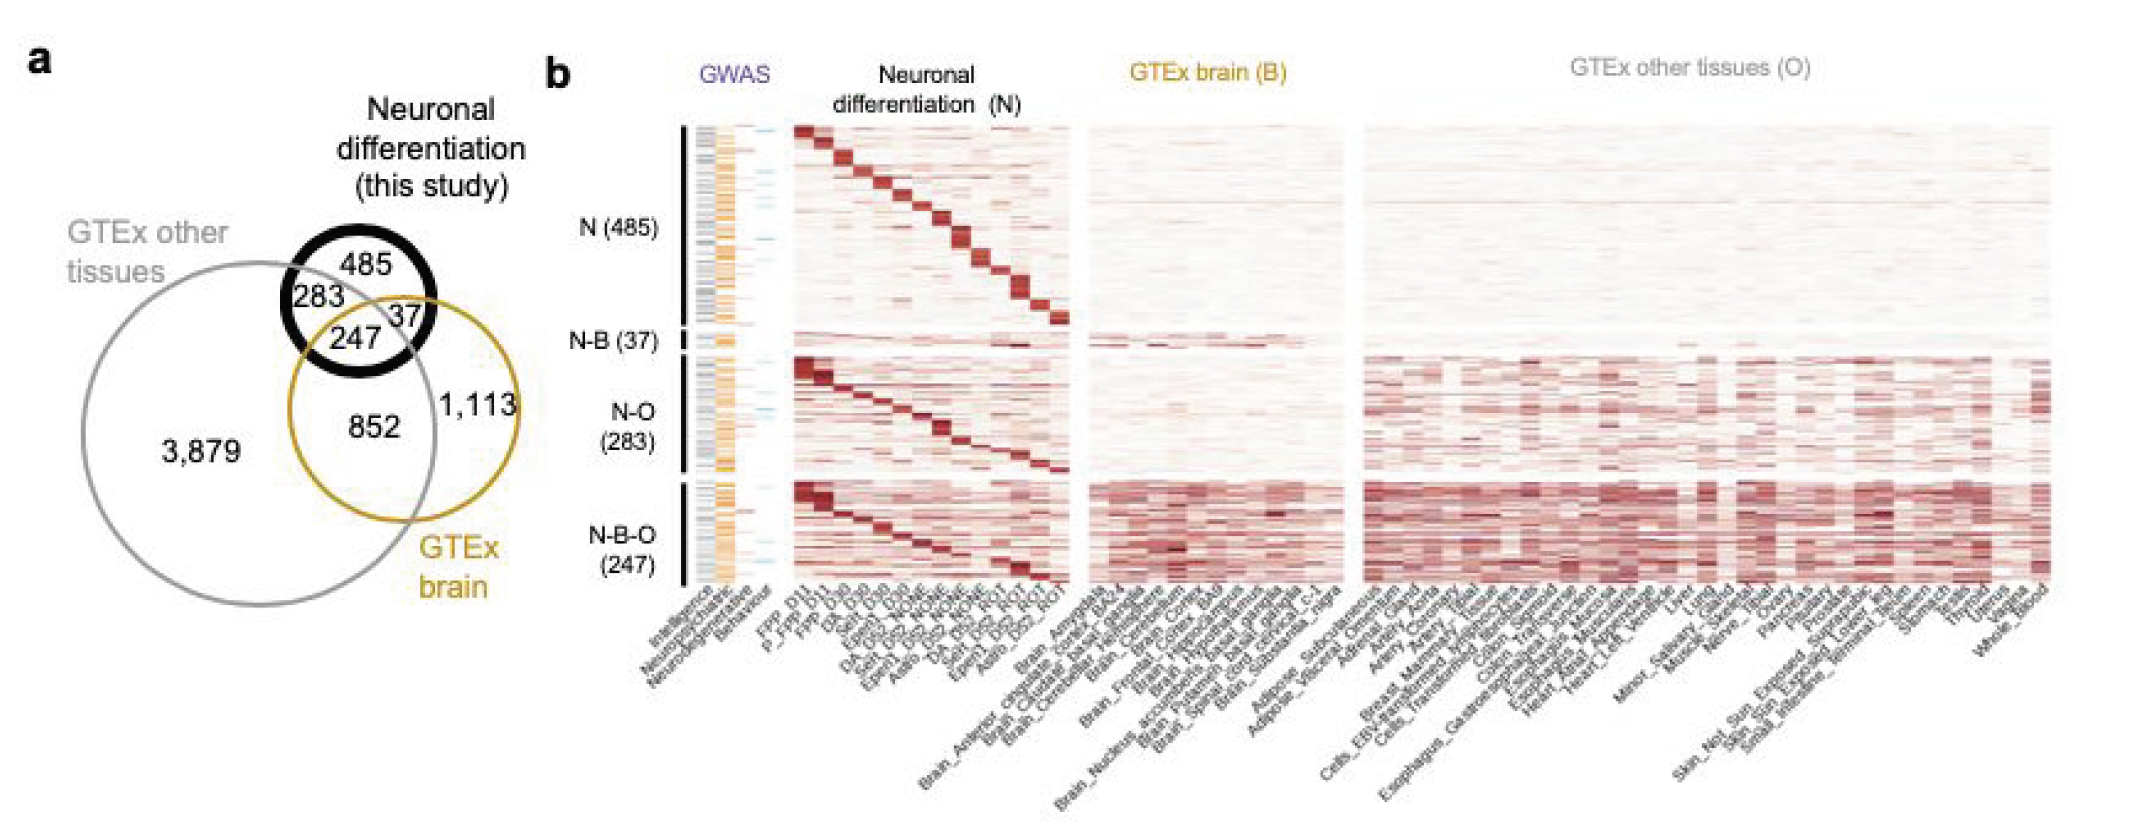
\includegraphics[width=16cm]{Chapter5/Fig/neuroseq_coloc_overview.png}
\caption[Coloc overview]{\textbf{Coloc overview}.\\
Overview of colocalisation analysis between our eQTL maps and 25 neuro-related GWAS traits. 
(left) Venn diagram showing the numbers of colocalisation events overlapping between our study, GTEx brain and GTEx non brain tissues. 
(right) Heatmap showing the posterior probability of colocalisation (PP4 from COLOC \cite{giambartolomei2014bayesian}) for our eQTL that colocalised with one or more GWAS traits. 
N: Neuronal differentiation (this study), B: GTEx Brain tissues, O: Other GTEx tissues.}
\label{fig:neuroseq_coloc_overview}
\end{figure}

\newpage

Among the most interesting colocalisation events was an eQTL for \textit{SFXN5}, a mitochondrial amino-acid transporter, which was specific to the rotenone-stimulated serotonergic neurons at day 52, and which colocalised with a Schizophrenia hit (PP4 = 0.78, \textbf{Fig. \ref{fig:neuroseq_coloc_example1}}). 
Exposure to rotenone is known to induce oxidative stress by inhibiting the mitochondrial respiratory chain complex I \cite{palmer1968studies, betarbet2000chronic}. 
We therefore speculate that the specific genetic signal observed for the mitochondrial gene \textit{SFXN5} in serotonergic neurons is a possible factor modulating environmental stress response.
% \\

\begin{figure}[h]
\centering
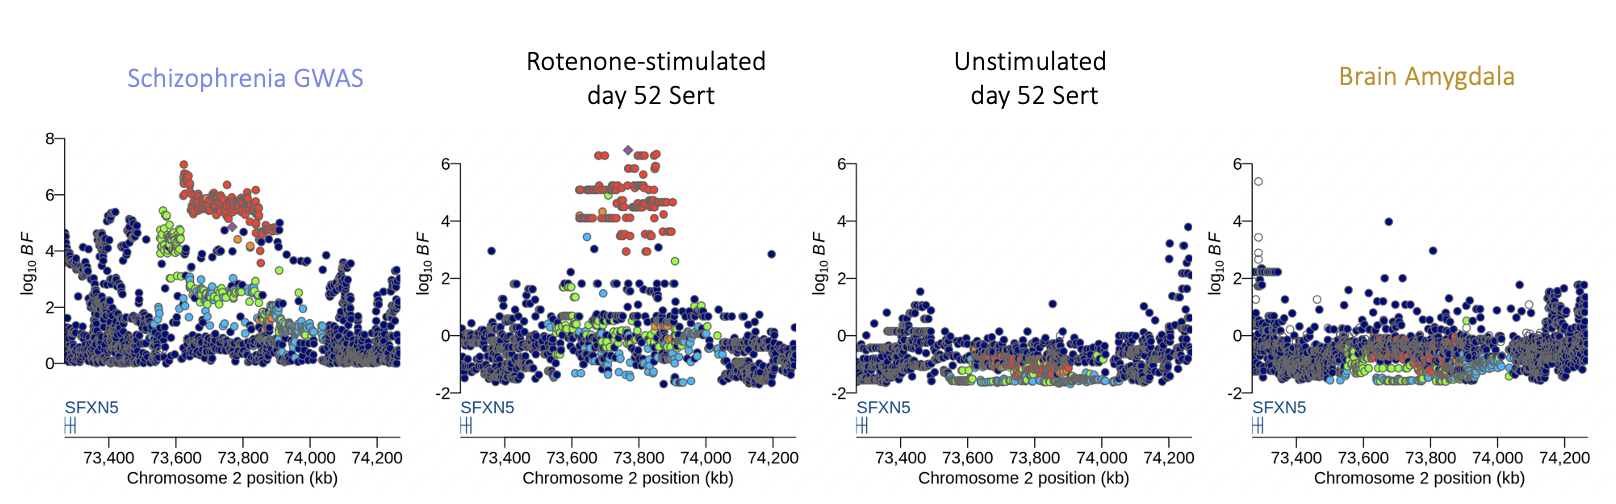
\includegraphics[width=15.5cm]{Chapter5/Fig/neuroseq_coloc_example1_SFXN5.png}
\caption[First example of colocalisation]{\textbf{A colocalisation event between a rotenone-specific eQTL and schizophrenia}.\\
Locus zoom plots around the \textit{SFXN5} gene. 
The Schizophrenia GWAS association (left) is colocalised with the eQTL in rotenone-stimulated serotonergic-like neurons at D52 (second panel from the left). 
No colocalisation signal was found in unstimulated serotonergic-like neurons at day 52 (third panel from the left) or any other brain GTEx tissues as illustrated here with GTEx Brain Amygdala (rightmost panel). 
The lead variant is indicated with a purple diamond and other points were coloured according to the LD index ($r^2$ value) with the lead variant.}
\label{fig:neuroseq_coloc_example1}
\end{figure}

Another example that colocalised with a Schizophrenia GWAS variant was an eQTL for
\textit{FGFR1}, detected both in proliferating and non proliferating floor plate progenitors at day 11 (PP4 = 0.93 and 0.88 respectively, \textbf{Fig \ref{fig:neuroseq_coloc_example2}}) . 
Previous studies have shown that nuclear \textit{FGFR1} plays a key role in regulating neural stem cell proliferation and central nervous system development, in part, by binding to the promoters of genes that control the transition from proliferation to cell differentiation \cite{ma2009molecular}. 
Additionally, it was shown that altered \textit{FGFR1} signaling was linked to the progression of the cortical malformation observed in schizophrenia \cite{stachowiak2017cerebral}.\\

\begin{figure}[h]
\centering
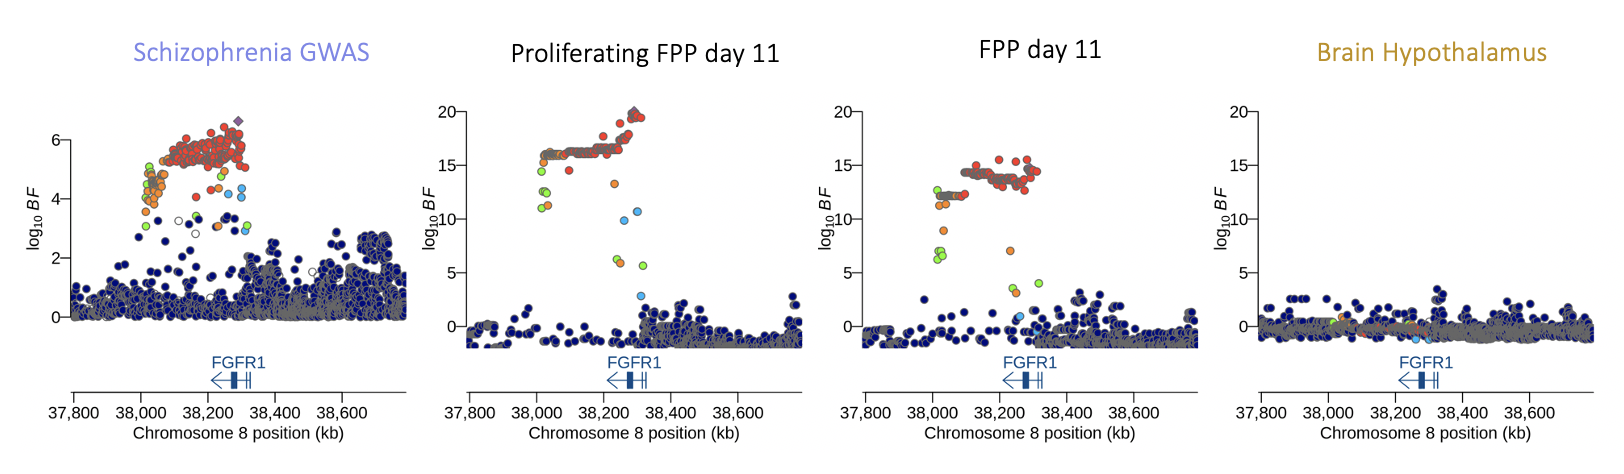
\includegraphics[width=15.5cm]{Chapter5/Fig/neuroseq_coloc_example2_FGFR1.png}
\caption[Second example of colocalisation]{\textbf{A schizophrenia colocalisation event with a developmental eQTL}.\\
A midbrain progenitor-specific eQTL for \textit{FGFR1} associated with schizophrenia. 
We identified a colocalisation event with this eQTL in both proliferating (second panel from the left) and non-proliferating floor plate progenitors (third panel from the left) at day 11. 
No colocalisation was found in any other cell type from our study (not shown) nor in any brain GTEx tissues (shown with GTEx Brain Hypothalamus, rightmost panel).}
\label{fig:neuroseq_coloc_example2}
\end{figure}

\newpage

These examples suggest that a combination of genetic and environmental factors during early development might contribute to schizophrenia pathology and illustrate how these data represent a valuable resource to understand the molecular basis of complex neurological diseases.

% add here discussion point on pseudobulk day 52?

% \clearpage

\section{Discussion}
\label{sec:neuroseq_discussion}

% this discussion needs re-writing, now it is basically copied from the paper

% disease relevance

% protocol efficiency

% cell type composition - joint model\\

The characterisation of the function of human trait-associated genetic variation requires large-scale studies, performed in disease-relevant cell types and states. 
Here, we demonstrate how human iPSCs can be efficiently profiled at scale throughout a 52 day-long differentiation to a midbrain neuronal cell fate. \\

First, we demonstrate high heterogeneity of cell types generated by this protocol (\textbf{Fig. \ref{fig:neuroseq_overview}}), and uncover a highly reproducible (\textbf{Fig. \ref{fig:neuroseq_diff_eff_replication}, \ref{fig:neuroseq_organoids}}), cell line-intrinsic neuronal differentiation bias (\textbf{Fig. \ref{fig:neuroseq_diff_efficiency}}).
Next, we show how this bias can be robustly predicted using gene expression profiling at iPSC state (\textbf{Fig. \ref{fig:neuroseq_ips_expression_signature}}). 
This is an important step towards the optimised design of future large-scale iPSC experiments, where cell lines can be rationally selected a priori without the need for laborious testing of differentiation capacity. \\

Indeed, the `quality' of human iPS cells has been carefully examined by several studies using both genetic and functional genomic data \cite{muller2011bioinformatic, international2018assessment, tsankov2015qpcr, bock2011reference}, see also \textbf{section
% 1.2.5
\ref{sec:ipsc_characterise}}. 
Despite these efforts, variation in differentiation potential between cell lines has been widely acknowledged, yet poorly understood. 
% % The underlying mechanisms have been hypothesised to involve epigenetic factors, environmental factors such as culture conditions, or changes acquired by cells over time in culture, or cell type of origin. 
To the best of our knowledge, the work we presented here is the first effort to systematically survey differentiation biases at the scale of an entire iPSC bank. 
To address this question, we leveraged the detailed phenotyping of cell lines in the HipSci bank.
We excluded the cell type of origin hypothesis \cite{hu2016effects} in this instance since all HipSci lines were derived from fibroblasts.
Moreover, we observed rather weak associations between neuronal differentiation efficiency and other biological factors, including X chromosome activation status, which has been described as relevant for other differentiation lineages (i.e. endoderm lineage, see \textbf{Chapter
\ref{chapter4}}
% 4
and \cite{cuomo2020single}).
% Instead, we found that variability in differentiation outcomes can be largely explained by cell-intrinsic factors that are maintained over multiple freeze/thaw cycles. 
% When we tested if these factors were due to the genetic variant inherited from the donor (\cite{kajiwara2012donor}), we found that a strong donor component was unlikely due to the poor
% correspondence in predicted differentiation outcomes between lines derived from the same individual. 
% Additionally, we did not detect significant effects in a genome-wide association analysis with predicted differentiation outcomes (p value > 5$\times 10^{-8}$, n = 540, MAF = 0.05). 
% Given these results, we suggest the two most likely candidates for future investigation are somatic genetic changes or persistent changes to cell line epigenomes that occur early in cellular reprogramming.
\\

Instead, our analysis indicates that the reduced production of neurons was best correlated with increased abundance of a specific subpopulation (cluster 2) of iPS cells that express the transcription factor \textit{UTF1} and other genes at elevated levels (\textbf{Fig. \ref{fig:neuroseq_ips_sc_genes}}).
Counter-intuitively, the proportion of cells in this subpopulation was positively correlated with the proportion of neuroblast cells on day 11, but lower fractions of dopaminergic and serotonergic-like neurons at later stages of differentiation. 
One possible explanation is that cell lines that commit earlier to a neuronal fate disproportionately lose neurons upon passaging at day 20 (\textbf{Fig. \ref{fig:neuroseq_experimental_design}}, cells are passaged at day 20 as from original protocol \cite{kriks2011dopamine}; this would explain the lack of clear differences between lines at day 11, with instead divergence appearing at the day 30 time point and then becoming even more evident by day 52).
% (why day 20?). 
\\

In alternative, cluster 2 may preferentially differentiate to radial glial cells which are more prone to switch to an astroglial and ependymal differentiation programme \cite{spassky2005adult}. 
In support of this hypothesis, we identified several genes that were up-regulated in cluster 2, including \textit{SIX3}, \textit{MT1F} and \textit{PITX2}, that are thought to play a role in astrocyte and ependymal cell biogenesis \cite{lavado2011six3, michael2011up, jacquet2009foxj1}. \\




% % this can probably be shortened, some can be moved to Chapter 7 even
% Indeed, the `quality' of human iPSCs has previously been carefully examined using both genetic and functional genomic data \cite{muller2011bioinformatic, international2018assessment, tsankov2015qpcr, bock2011reference}, see also section \ref{sec:ipsc_characterise}. 
% Despite these efforts, differentiation bias among cell lines has been widely appreciated, yet poorly understood. 
% % The underlying mechanisms have been hypothesised to involve epigenetic factors, environmental factors such as culture conditions, or changes acquired by cells over time in culture, or cell type of origin. 
% To the best of our knowledge, the work presented here is the first to systematically survey differentiation biases at the scale of an entire cell bank. 
% To address this question, we leveraged the large number of cells in the HipSci bank and the detailed phenotyping of each of these lines. 
% We excluded the cell type of origin hypothesis \cite{hu2016effects} in this instance since all HipSci lines were skin-derived.
% We also observed relatively weak relationships between neural differentiation efficiency and other biological factors, such as X chromosome inactivation status, which has been described as relevant for other differentiation lineages (i.e. endoderm lineage, see Chapter
% % \ref{chapter4}
% 4 and \cite{cuomo2020single}).
% Instead, we found that variability in differentiation outcomes can be largely explained by cell-intrinsic factors that are maintained over multiple freeze/thaw cycles. 
% When we tested if these factors were due to the genetic variant inherited from the donor (\cite{kajiwara2012donor}), we found that a strong donor component was unlikely due to the poor
% correspondence in predicted differentiation outcomes between lines derived from the same individual. 
% Additionally, we did not detect significant effects in a genome-wide association analysis with predicted differentiation outcomes (p value > 5$\times 10^{-8}$, n = 540, MAF = 0.05). 
% Given these results, we suggest the two most likely candidates for future investigation are somatic genetic changes or persistent changes to cell line epigenomes that occur early in cellular reprogramming.\\

% In particular, our analysis indicates that the reduced production of neurons was best
% correlated with increased abundance of a specific subpopulation (cluster 2) of iPS cells that express the transcription factor UTF1 and other genes at elevated levels (Fig. \ref{fig:neuroseq_ips_sc_genes}).
% Counter-intuitively, the proportion of cells in this subpopulation was positively correlated with the proportion of neuroblast cells on day 11, but lower fractions of dopaminergic and serotonergic neurons at later stages of differentiation. 
% One possible explanation is that cell lines that commit earlier to a neuronal fate disproportionately lose neurons upon passaging at day 20. 
% Alternatively, cluster 2 may preferentially give rise to radial glial cells that more readily switch to an astroglial and ependymal differentiation programme \cite{spassky2005adult}. 
% In support of this hypothesis, we identified several upregulated genes in cluster 2, including \textit{SIX3}, \textit{MT1F} and \textit{PITX2}, that are thought to play a role in astrocyte and ependymal cell biogenesis \cite{lavado2011six3, michael2011up, jacquet2009foxj1}. 
% We speculate that culture methods that reduce iPSC heterogeneity may reduce the fraction of iPSC lines that resist efficient neuronal differentiation. 
% We also note that our findings do not explain all of the variance in neuronal differentiation capacity, and future studies will be required to more fully understand the biological basis of the differentiation bias we have observed here.\\

% Based on molecular markers that are predictive for differentiation bias, we could estimate that 16\% of iPSC lines in the HipSci resource produce few to no identifiable neuronal cell types under the conditions tested. 
% While the production of neuronal cells was intrinsically limited in these cell lines, the fact that this effect was associated with particular cell lines but not with particular donors suggests that cell banks that contain multiple lines per donor can be most effectively utilised for applications involving neural differentiation by the rational selection of cell clones. 
% Importantly, this a priori selection is enabled by gene expression profiling data from the pluripotent state that is easily obtainable and often already available.\\


A second implication of our study is that, despite growth competition between cell lines, pooled experiments retain sufficient cells per donor to carry out genetic analysis, even following extended periods in culture. 
Although cells from different lines were pooled in similar numbers, we observed extensive variation throughout our differentiation experiments in the numbers of cells produced by different lines. 
% mavbe also highlgiht that this needs to be taken into account when mapping QTL…
For example, 50\% of the cells we sequenced were produced by only 12\% of lines.
As we have demonstrated, this was an important effect to take into account in our eQTL analysis (\textbf{Fig. \ref{fig:neuroseq_eqtl_improved_power}}).
Future technical improvements, for instance more precise matching of growth rates of cell lines within pools, or line selection based on predicted differentiation efficiency using markers in the iPSC state may further increase the utility of multiplexed iPSC differentiation experiments.\\

% % in contrast, lengthen this second part on eQTL

% Thirdly, 
Finally,
we could map eQTL across several neuronal cell types and in response to oxidative stress (\textbf{Fig. \ref{fig:neuroseq_eqtl}}).
As we have seen, in order to understand the functional role of trait-associated variants it is crucial to perform genetic analyses in relevant cell types.
Indeed, as a community, we have largely been unable to identify genetic variants that drive expression changes in narrowly-defined cell populations.
% rephrase
This is due to our reliance on tissue-level data (e.g. GTEx), our incomplete knowledge of cell populations present in a tissue, or because rare cell populations do not provide enough substrate for common genomics assays. \\

Our analysis attempts to be a step towards investigating cell type-specific genetic effect, which are often masked in tissue-level assays.
% identified several hundred trait-associated genetic changes in gene expression that have not been previously identified. 
Indeed, despite a modest sample size, our study reveals a disproportionately large number of novel colocalisations between neurological traits and diseases and eQTL (\textbf{Fig. \ref{fig:neuroseq_coloc_overview}}) compared with GTEx tissues of equivalent sample size. 
For example, the number of novel trait/disease-eQTL colocalisations added by GTEx liver or cerebellar hemisphere (n=208, 215 respectively) are 80 and 107, respectively, compared to 597 in this study. 
A simple explanation for this result is that our experiment profiled expression states that are hard to capture using post-mortem tissue, including time points during neuronal differentiation and rotenone exposure. \\

Additionally, the single-cell resolution of our study enabled the detection of many eQTL that were specific to individual cell types, or could only be detected upon stimulation (\textbf{Fig. \ref{fig:neuroseq_eqtl_examples}}).
These signals, while present, are challenging to detect in bulk tissue because the relevant cell types are often rare. 
Combined, these results suggest that many `missing', disease-relevant eQTL remain to be discovered using single cell profiling of both primary tissues and \textit{in vitro} models.\\

% Overall, our study demonstrates the utility of pooled iPSC differentiation and single-cell analysis for revealing the function of disease-associated genetic variation in otherwise inaccessible cell states. \\


% JCM: A bit like the final paragraph of a paper rather than thesis chapter.
% In summary, work presented in this chapter clearly demonstrates how iPSC differentiation combined with single cell RNA-seq profiling unlocks population-level studies in increasingly complex, dynamic and biologically realistic cellular models. 
% We anticipate that future uses of this model system will focus on experimental settings that are challenging or impossible with primary cells. 
% These may include single cell resolution sampling along longer differentiation times to more complex differentiation trajectories, such as cell organoids, or involve large panels of disease relevant-stimuli and drug exposures. 
% Collectively, our study will guide future efforts to understand the common genetic basis of neurological disorders, and facilitate the development of iPSC-based approaches for modelling and treating these diseases. \\

% As population-scale studies across more and more complex cellular models, assayed using single cell transcriptomics, become available, there is increasing need for joint models for eQTL mapping that account for multiple sources of cellular heterogeneity. 
% In the next chapter (\textbf{Chapter 
% \ref{chapter6}}),
% % 6), 
% I present a  novel method that allows to jointly map multi-context eQTL across several cell states and types at single cell resolution.

% In the next chapter, \textbf{Chapter \ref{chapter7}}, I provide an outlook..